%\documentclass[a4paper,fleqn,longmktitle]{cas-dc}
\documentclass[a4paper,fleqn]{cas-dc}
%\usepackage{l3regex}

\usepackage{lipsum}
\usepackage{graphicx}
\usepackage{graphicx}
\usepackage{multirow}
\usepackage{caption}
\usepackage{booktabs}
\usepackage{color, colortbl}
%\usepackage[table]{xcolor}
\usepackage{float}
\usepackage{lipsum}
\newcommand\mycorrections[1]{\textcolor{red}{#1}}
\newcommand\mycorrectiong[1]{\textcolor{green}{#1}}
\newcommand\mycorrectiony[1]{\textcolor{yellow}{#1}}
%\usepackage[authoryear,longnamesfirst]{natbib}
\usepackage[numbers]{natbib}

\xspaceaddexceptions{]}
\def\tsc#1{\csdef{#1}{\textsc{\lowercase{#1}}\xspace}}
%\tsc{WGM}
%\tsc{QE}
%\tsc{EP}
%\tsc{PMS}
%\tsc{BEC}
%\tsc{DE}


\begin{document}
\let\WriteBookmarks\relax
\def\floatpagepagefraction{1}
\def\textpagefraction{.001}
\shorttitle{Fuel consumption Anomaly detection }
\shortauthors{Mulongo et al.}
%\begin{frontmatter}

\title [mode = title]{Machine Learning in Fuel Consumption II: An Anomaly Detection Approach in Power Generation Plants}                      
%\tnotemark[1,2]

%%  \tnoteref{tn1,tn2}

%\tnotetext[1]{This document is the results of the research
%   project funded by the National Science Foundation.}

%\tnotetext[2]{The second title footnote which is a longer text matter
%   to fill through the whole text width and overflow into
%   another line in the footnotes area of the first page.}



\author[1]{J.Mulongo}[type=editor,
                        auid=000,bioid=1,
                        %prefix=Sir,
                        %role=Researcher,
                        orcid=0000-0001-7511-2910]
\cormark[1]
%\fnmark[1]
\ead{jecinta.mulongo@aims-cameroon.org}
%\ead[url]{www.cvr.cc, cvr@sayahna.org}

\credit{Conceptualization of this study, Methodology, Software}

\address[1]{Mathematical Sciences (AIMS-Cameroon)}



\author[2,3]{T. Ansah-Narh}
   %role=Co-ordinator,]
\cormark[2]
%\fnmark[1]
\ead{t.narh@gaecgh.org}

\author[4]{M. Atemkeng}[%
role=Co-ordinator,
prefix=Dr,
]
%\fnmark[4]
\ead{m.atemkeng@gmail.com}
%\ead[URL]{www.sayahna.org}

%\credit{Data curation, Writing - Original draft preparation}

\address[2]{Centre for Radio Astronomy \& Astrophysics, Ghana Space Science and Technology Institute, Ghana Atomic Energy Commission, P. O. Box LG 80, Legon - Accra, Ghana}

\author[5]{Rockefeller}
%\cormark[2]
%\fnmark[1,3]
\ead{rockefeller@aims-senegal.org}

\author[4] {M. Garuti}[]
%
\cormark[2]
%\fnmark[1,3]
\ead{marco@aims-cameroon.org}
%\ead[URL]{www.stmdocs.in}

\address[3]{Space \& Atmospheric Research Group, Ghana Space Science and Technology Institute, Ghana Atomic Energy Commission, P. O. Box LG 80, Legon - Accra, Ghana}

\address[4]{Rhodes Centre for Radio Astronomy Techniques \& Technologies(RATT)}
\address[5]{Mathematical Sciences (AIMS-Senegal)}
\cortext[cor1]{Corresponding author}
\cortext[cor2]{Principal corresponding author}

\cortext[cor1]{Corresponding author}
\cortext[cor2]{Principal corresponding author}
%\fntext[fn1]{This is the first author footnote. but is common to third
%  author as well.}
%\fntext[fn2]{Another author footnote, this is a very long footnote and
%  it should be a really long footnote. But this footnote is not yet
%  sufficiently long enough to make two lines of footnote text.}

%\nonumnote{This note has no numbers. In this work we demonstrate $a_b$
%  the formation Y\_1 of a new type of polariton on the interface
%  between a cuprous oxide slab and a polystyrene micro-sphere placed
%  on the slab. The evanescent field of the resonant whispering gallery
%  mode (\WGM) of the micro sphere has a substantial gradient, and
%  therefore effectively couples with the quadrupole $1S$ excitons in
%  cuprous oxide.
%  \lipsum[1]
%  }

\begin{abstract}[S U M M A R Y]
High fuel consumption is experienced in \mycorrections{ telecommunication} based stations. As telecommunication base stations require electricity to operate, high fuel consumptions remains a challenge in base stations management as the working capital increases every year. To cope with this problem, we aim to detect anomalies in the recorded data by learning the pattern of the fuel consumed dataset and compare the performance of the four classification techniques on the unseen dataset. In this paper, we show the use of supervised machine learning classification based techniques in detecting anomalies associated with the fuel consumed dataset from TeleInfra\footnote{{\tt http://www.art.cm/en/node/3111}} base station using the generator as a source of power. We made use of machine learning techniques to train the dataset, these include support vector machines (SVM), k-nearest neighbor (KNN), logistic regression (LR), and multilayer perceptron (MLP).  We evaluate models performance using K-fold
cross validation and training test split techniques and classification performance metrics were used to evaluate the fitted models. Comparative study of the classifier is done for model selection, and the result of this study shows that MLP has the best performance in the evaluation measured used with a score of $0.96$ in both K-fold cross validation and train test split. In the area under the receiver operating characteristic and precision-recall curve, the model attained a score of $1.00$ and $0.98$ respectively. Our results also show that the working hours of the generator explains much the classification class. 
\end{abstract}
\begin{keywords}
Anomalies \sep Multilayer  Perceptron \sep K-Nearest Neighbor   \sep Support Vector Machines \sep Logistic Regression\sep Machine Learning \sep Classification
\end{keywords}


\maketitle

\section{Introduction}

The expansion of mobile services of the telecommunication industries has resulted in the installation of cell towers to diverse parts of the world. In developing countries like Cameroon, the supply of the power grid is irregular and the network companies find it difficult to manage their base stations particularly, their data centers and other IT equipment\mycorrections{s}. Due to this, the management of the base stations uses diesel generators, solar panels, batteries and another secondary source of power as a backup plan to keep running their systems. However, these other power sources have also generated other problem, specifically, fuel pilferage from those who have access to fuel distribution in the various base stations and also, from other people in the vicinity and high fuel consumption as a result of the generator malfunctioning.

With an objective to provide base station management service such as refueling and site maintenance, TeleInfra\footnote{{\tt http://www.art.cm/en/node/3111}} company in Cameroon faces the problem of electricity shortage\mycorrections{,}hence\mycorrections{,} the company had a generator as an alternative source of power. The company works with an objective is to provide management services such as site maintenance and refueling of generators in the base stations. Like any other power dependence company in Africa, 
the company faces the problem of electricity shortages and hence, chooses to have a generator as a main back up plan. The main goal of this paper is to use machine learning (ML) \mycorrections{algorithms} to learn the pattern of the fuel consumed by generator power plants in the 
TeleInfra\footnote{{\tt http://www.art.cm/en/node/3111}} company in order to observe some outliers produced by the system. The dataset used in this paper is obtained from  base stations  under supervision of TeleInfra company. It contains attributes of fuel consumed by the generators and other informations such as maintenance details.

Anomaly in a data is considered as an observation which do not conform to the expected standard in the data. Meanwhile, recent works in anomaly detection such as fraud detection analysis~\citep{2017arXiv170601953Z, chouiekh2018convnets}, 
thermal power plant~\citep{banjanovic2017neural}, medical image analysis~\citep{taboada2009anomaly}, etc., have shown how well ML techniques can be used to address these challenges.
% \indent 
From the various anomalies detection research, the algorithms used can outperform each other based on the type of data 
and the underlying assumptions employed. From the literature, most of the competitive ML techniques used in classification task like in our case, consist of SVM, KNN, LR, and MLP. In this study, we do a comparative analysis of the performance of these classifiers to determine the best classifier that can accurately detect the anomalies in the fuel consumption dataset. SVM aims in generating an optimal hyperplane that maximizes the margin between two class\mycorrections{es}, that is, in the case linearly separable binary classification whereas KNN  stores the training data and predict the test instance based on distance measure and the majority votes from the training sample. LR uses probabilities to predict the chance of a sample to belong in a certain class. MLP learns the complexity of data and optimizes the weights to minimize classification error. A more detailed explanation of these classifiers is given in Section~\ref{sec:med}.


%The rest of this paper is organized as follows: Section \ref{sec:expl} describe the dataset, feature selection and descriptive findings from the data. Section \ref{sec:med} we describe machine learning methods used in the study. Section \ref{sec:resu} we conclude the results and finding from the study discussed with comparative analysis performance of the methods used.
\mycorrections{The rest of this paper is organized as follows: Section \ref{sec:expl} we describe the dataset used in the study, data preprocessing conducted and exploratory data analysis. In Section \ref{sec:med} we provide a brief description of machine learning algorithms and evaluation metrics used to perform model selection. Section \ref{sec:resu} gives the result of the evaluation matrices capabilities in predicting whether an input is an anomaly or normal consumption.}



\section{EXPLORATORY DATA ANALYSIS}  \label{sec:expl}

\subsection{Dataset} \label{sec:desc}

The dataset is collected by cell site management company is Cameroon; TeleInfra\footnote{{\tt http://www.art.cm/en/node/3111}}. The dataset contained different power type used by telecommunication cell site and we mainly focus on base stations powered by the generator. We limited to this kind of dataset as our major goal is to identify the cause of high fuel consumption by performing anomaly detection. It has 32 features both numerical and categorical data with a sample size of $5905$ inputs of the fuel consumed within September $2017$ to September $2018$. Variables description is given by Table \ref{Variables} in Section \ref{appendix}. The missing observation which accounts to $1.75\%$ of the full dataset were dropped to reduce the assumption made on the data by replacing. The variables used to fit the models were rescaled to ensure all the features have the same treatment. The dataset contains details of fuel consumed by generator and maintenance report made on the generator. This information recorded includes the working hours of the generator, the rate of consumption, fuel consumed, the quantity of fuel added in the generator, e.t.c.

From the $16$ variables associated with fuel consumption, we extracted the variables that give more information about the output class. 
The important features used to fit the models were selected using the
Gradient Boosting Classifier (GBC) to reduce the number of features that do not impact the model performance. We preferred GBC to fit our dataset feature importance due to its ability to minimize bias and overfitting. This has been achieved in gradient boosting at error correction which is done based at every stage hence optimizing the objective function.

Figure \ref{fig:feature} shows that the variable\\ \textit{RUNNING\_TIME\_PER\_DAY} of the generator is the key important feature which has a great influence on the output. We also understand from Figure \ref{fig:rr} the generator is working per day has a positive correlation with fuel consumed which explains why an increase in the running hours of the generator increases fuel consumption. \textit{DAILY\_CONSUMPTION}  and \textit{CONSUMPTION\_HIS} variables give the fuel consumed per day and fuel consumed per period before the next refueling is done respectively. Other features such as \textit{MAXIMUM\_CONSUMPTION\_PER\_DAY}, the \textit{CONSUMPTION\_RATE }, \textit{QTE\_FUEL\_FOUND} e.t.c, have less information about the classification output class. The variables considered to fit the model included variables with at least $20\%$ relative importance. Figure \ref{fig:feature} shows feature importance fitted using Gradient Boosting classifier.

\begin{figure}
		\begin{minipage}[H]{\linewidth}
	\centering
	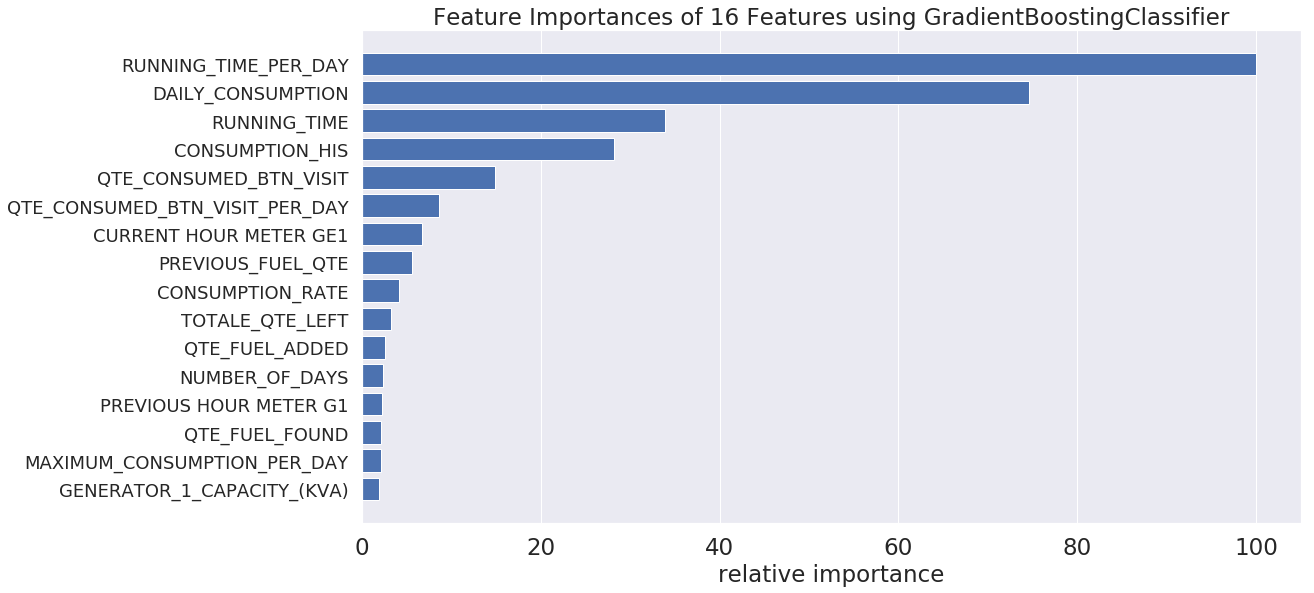
\includegraphics[width=1.1\textwidth]{Figures/Feature_importance.png} 
		\end{minipage}
	\caption{Feature importance ranking fitted using Gradient Boosting classifier }
	\label{fig:feature}
	
\end{figure} 
From a total sample of $5905$, $35.11$\%  of the sample were \mycorrections{ manually labeled} as anomaly class and the rest as a normal class. The classification classes labeling was done based on the anomalies observed in the dataset.  Anomalies in the data observed include outliers, wrong entry on the number of hours the generator was working in a day, consumption per day exceeding maximum consumption the generator can take in a day and generator fuel reducing when the generator was not working. All these observations were considered to label the classification class as either normal consumption or anomaly. 

Class imbalance is a problem that highly affects classification base task. This is where the number of one class is significantly large compared to the other class. The effects of class imbalance are seen in the performance measure such as accuracy whose computation depends on both classes i.e., normal and anomaly class \cite{awoyemi2017credit}. A corrective measure of class imbalance has been proposed, that is, the use of sampling method \cite{brownlee2016master}. Sampling method can be classified as either undersampling or oversampling. \mycorrections{In the case of the oversampling method, classification class with small sample size is increased by generating a duplicate of the existing sample. This is done to ensure class attains the same sample size as the majority class. Undersampling takes the reverse of oversampling where the classification class which represent the majority is reduced in number to have both classification classes to have an equal sample size.} 

Oversampling methods involves duplicating minority class to add more inputs so as to have equal sample size as to that class with the majority sample. On the other side, undersampling involves reducing the majority of data to have the same sample size as a minority.

\subsection{Descriptive Analysis}

Figure \ref{fig:probitplot} shows the probability frequency distribution of the fuel consumed. The fuel consumed by generator has asymmetry normal distribution with mean $261.80$ and standard deviation of $175.06$. Large variance is as a result of dispersion and the skewness of the fuel consumed data. Classifiers assume the underlying distribution of the dataset hence the distribution has a great impact on the performance of classifiers \cite{japkowicz2011evaluating}. 
Figure \ref{fig:probitplot} shows the kernel density estimation and normal probability plot for the fuel consumed dataset. 
\begin{figure}
	\begin{minipage}[H]{\linewidth}
	\centering
	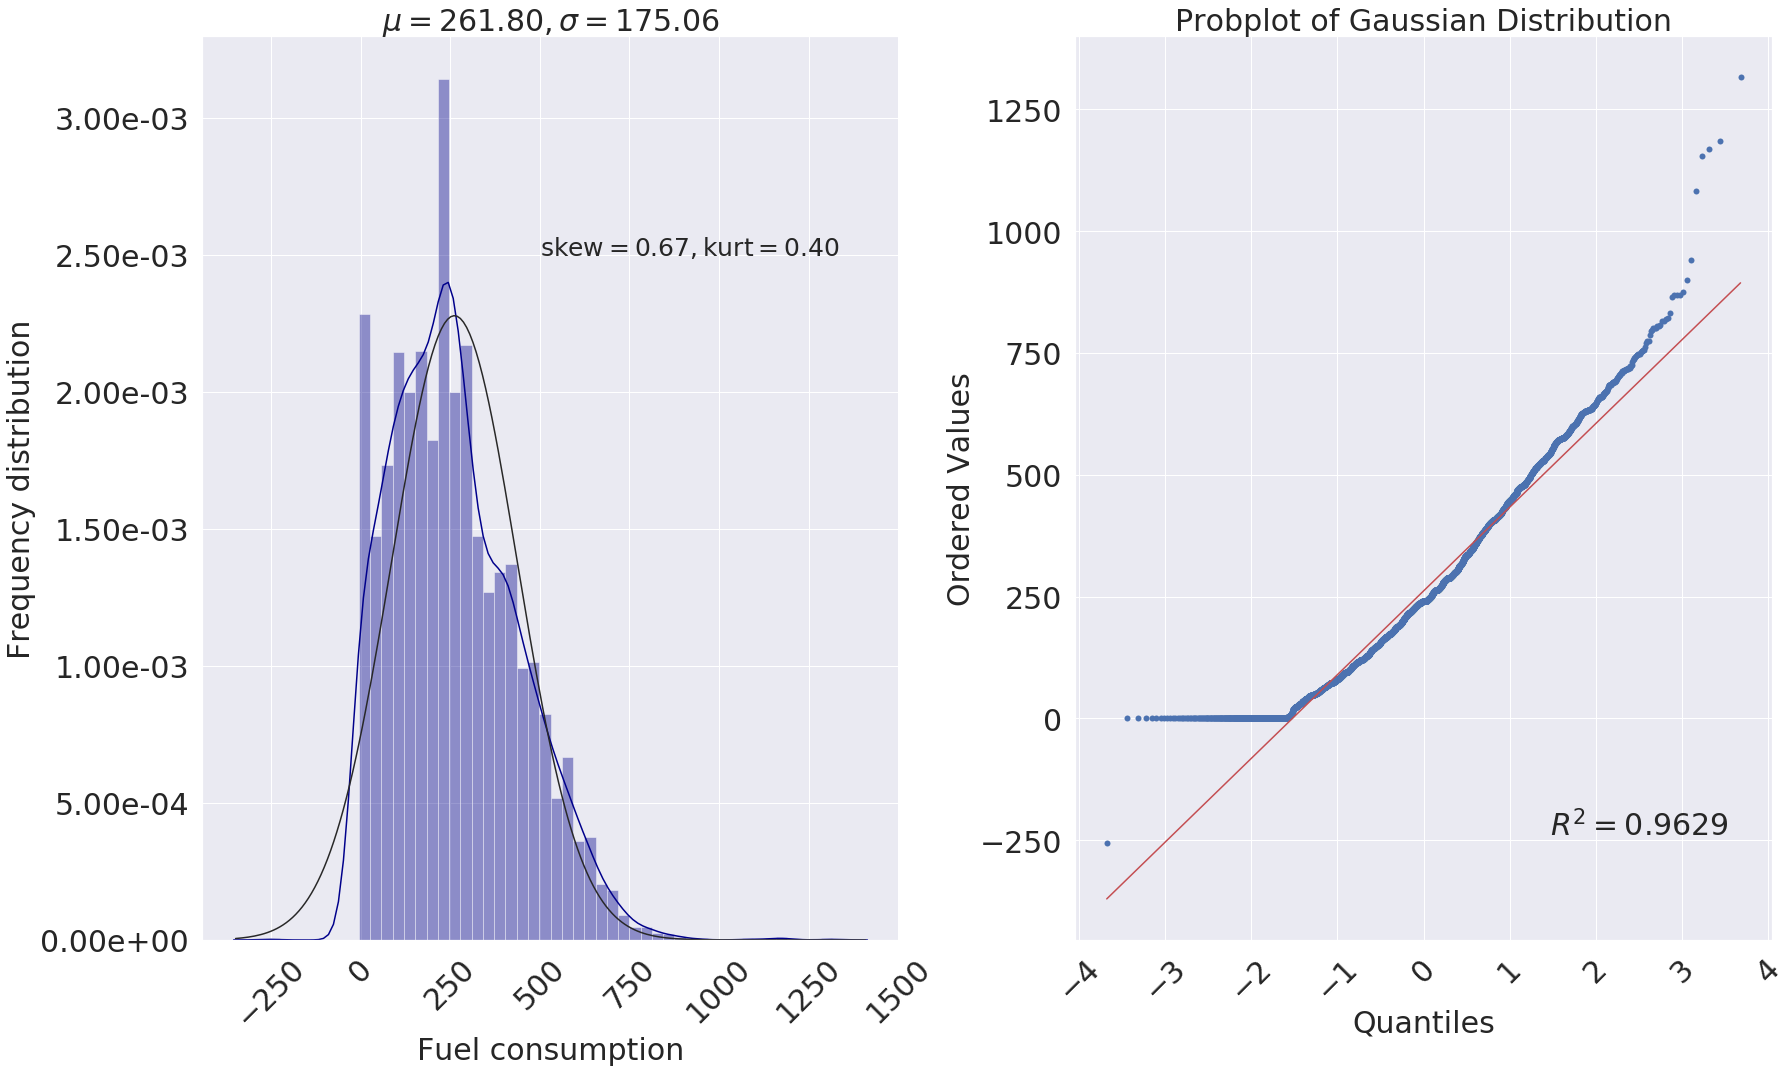
\includegraphics[width=1.0\linewidth]{Figures/probitPlot}
\end{minipage}
	\caption{Average distribution of the fuel consumed}
	\label{fig:probitplot}
\end{figure}

%
%\begin{figure*}
%   \begin{minipage}[H]{\linewidth}
%      \centering
%      \includegraphics[width=1.0\textwidth]{fig/normalcurve} %
%    \end{minipage}
%     \caption{Average distribution of the fuel consumed}
%    \label{fig:normalcurve}
%   \end{figure*}

% \begin{figure}[tbph]
% 	\centering
% 	\includegraphics[width=1.2\linewidth]{normalcurve}
% 	\caption{Kernel density estimation and Gaussian distribution of fuel consumed}
% 	\label{fig:normalcurve}
% \end{figure}\\
%From the work done by \cite{maxime2018} on prediction of fuel consumption on the same dataset with all anomalies put into consideration, the mean of the fuel consumed within the period is $289.04$ litters with a standard deviation of $160.09$. The mean improvement is a result of the zero consumption and fuel consumption with anomalies  not taken into consideration.

\mycorrections{ Anomalies in the data provide a wrong estimate of the fuel consumed. Considering all the anomalies we observed in the data, the normal consumption observation was used to make the prediction of the estimated fuel consumed \cite{maxime2018}. From the normal consumed dataset, we observed that the mean and the standard deviations were $289.04$(L) and $160.09$ respectively.
	Figure \ref{fig:probitplot} shows the Gaussian distribution plot which indicates that the dataset has outliers, as a result of this, the normal distribution curve deviating from the mean. Zero consumption of fuel consumed entries in the dataset causes the normal curve to start above the normal line. This explains the positive skewness of the fuel consumed with a skew of  $0.40$. Due to the high number of the zero consumption in the data as shown in Figure \ref{fig:probitplot}, observations with this characteristics were considered as an anomaly in the case where fuel reduced in the generator tank despite having zero consumption. 
}
% Due to this, the zero consumption samples were compared with the difference between what was left in the generator previously visit and what was found in the generator to make sure that consumption was actually zero fuel. As a result of the outliers, the normal distribution curve of the fuel consumed is shifted to the left, this contributes to the skew distribution of the fuel consumed. 

Figure \ref{fig:correlation matrix} displays a correlation matrix between numerical variables in the dataset. 
Correlation is a normalized covariance with its values ranges from $-1$ to $1$. The matrix measures a linear relationship between variables with $-1$ \mycorrections{indicating that} two variables have a strong negative relationship, that is, as one variable increases, the other one decreases and $1$ indicates strong positive relation, that is, an increase in one variable results to increase in the other one. The diagonal values indicate the correlation of a variable with itself. \mycorrections{ It can be seen from From Figure \ref{fig:correlation matrix} that the} fuel consumed have strong positive relation of $0.83$ with the number of hours the generator is working. \mycorrections{ The strong positive correction explained the dependence of the fuel consumed on the number of hours the generator is working and the rate of consumption of the generator. The two variables determine the quantity consumed. }
The quantity of fuel added and the fuel consumed has a positive correlation coefficient of $0.14$. The rate at which the generator consumes fuel has a positive correlation of $0.31$ with the consumption. The classification class which is the output variable has also positive correction of $0.027$  with fuel consumed. The correlation matrix provides the linear relationship existing between variables but it does not explain in the case where the variables have a non-linear relation.

\begin{figure}
	\begin{minipage}[H]{\linewidth}
	\centering
	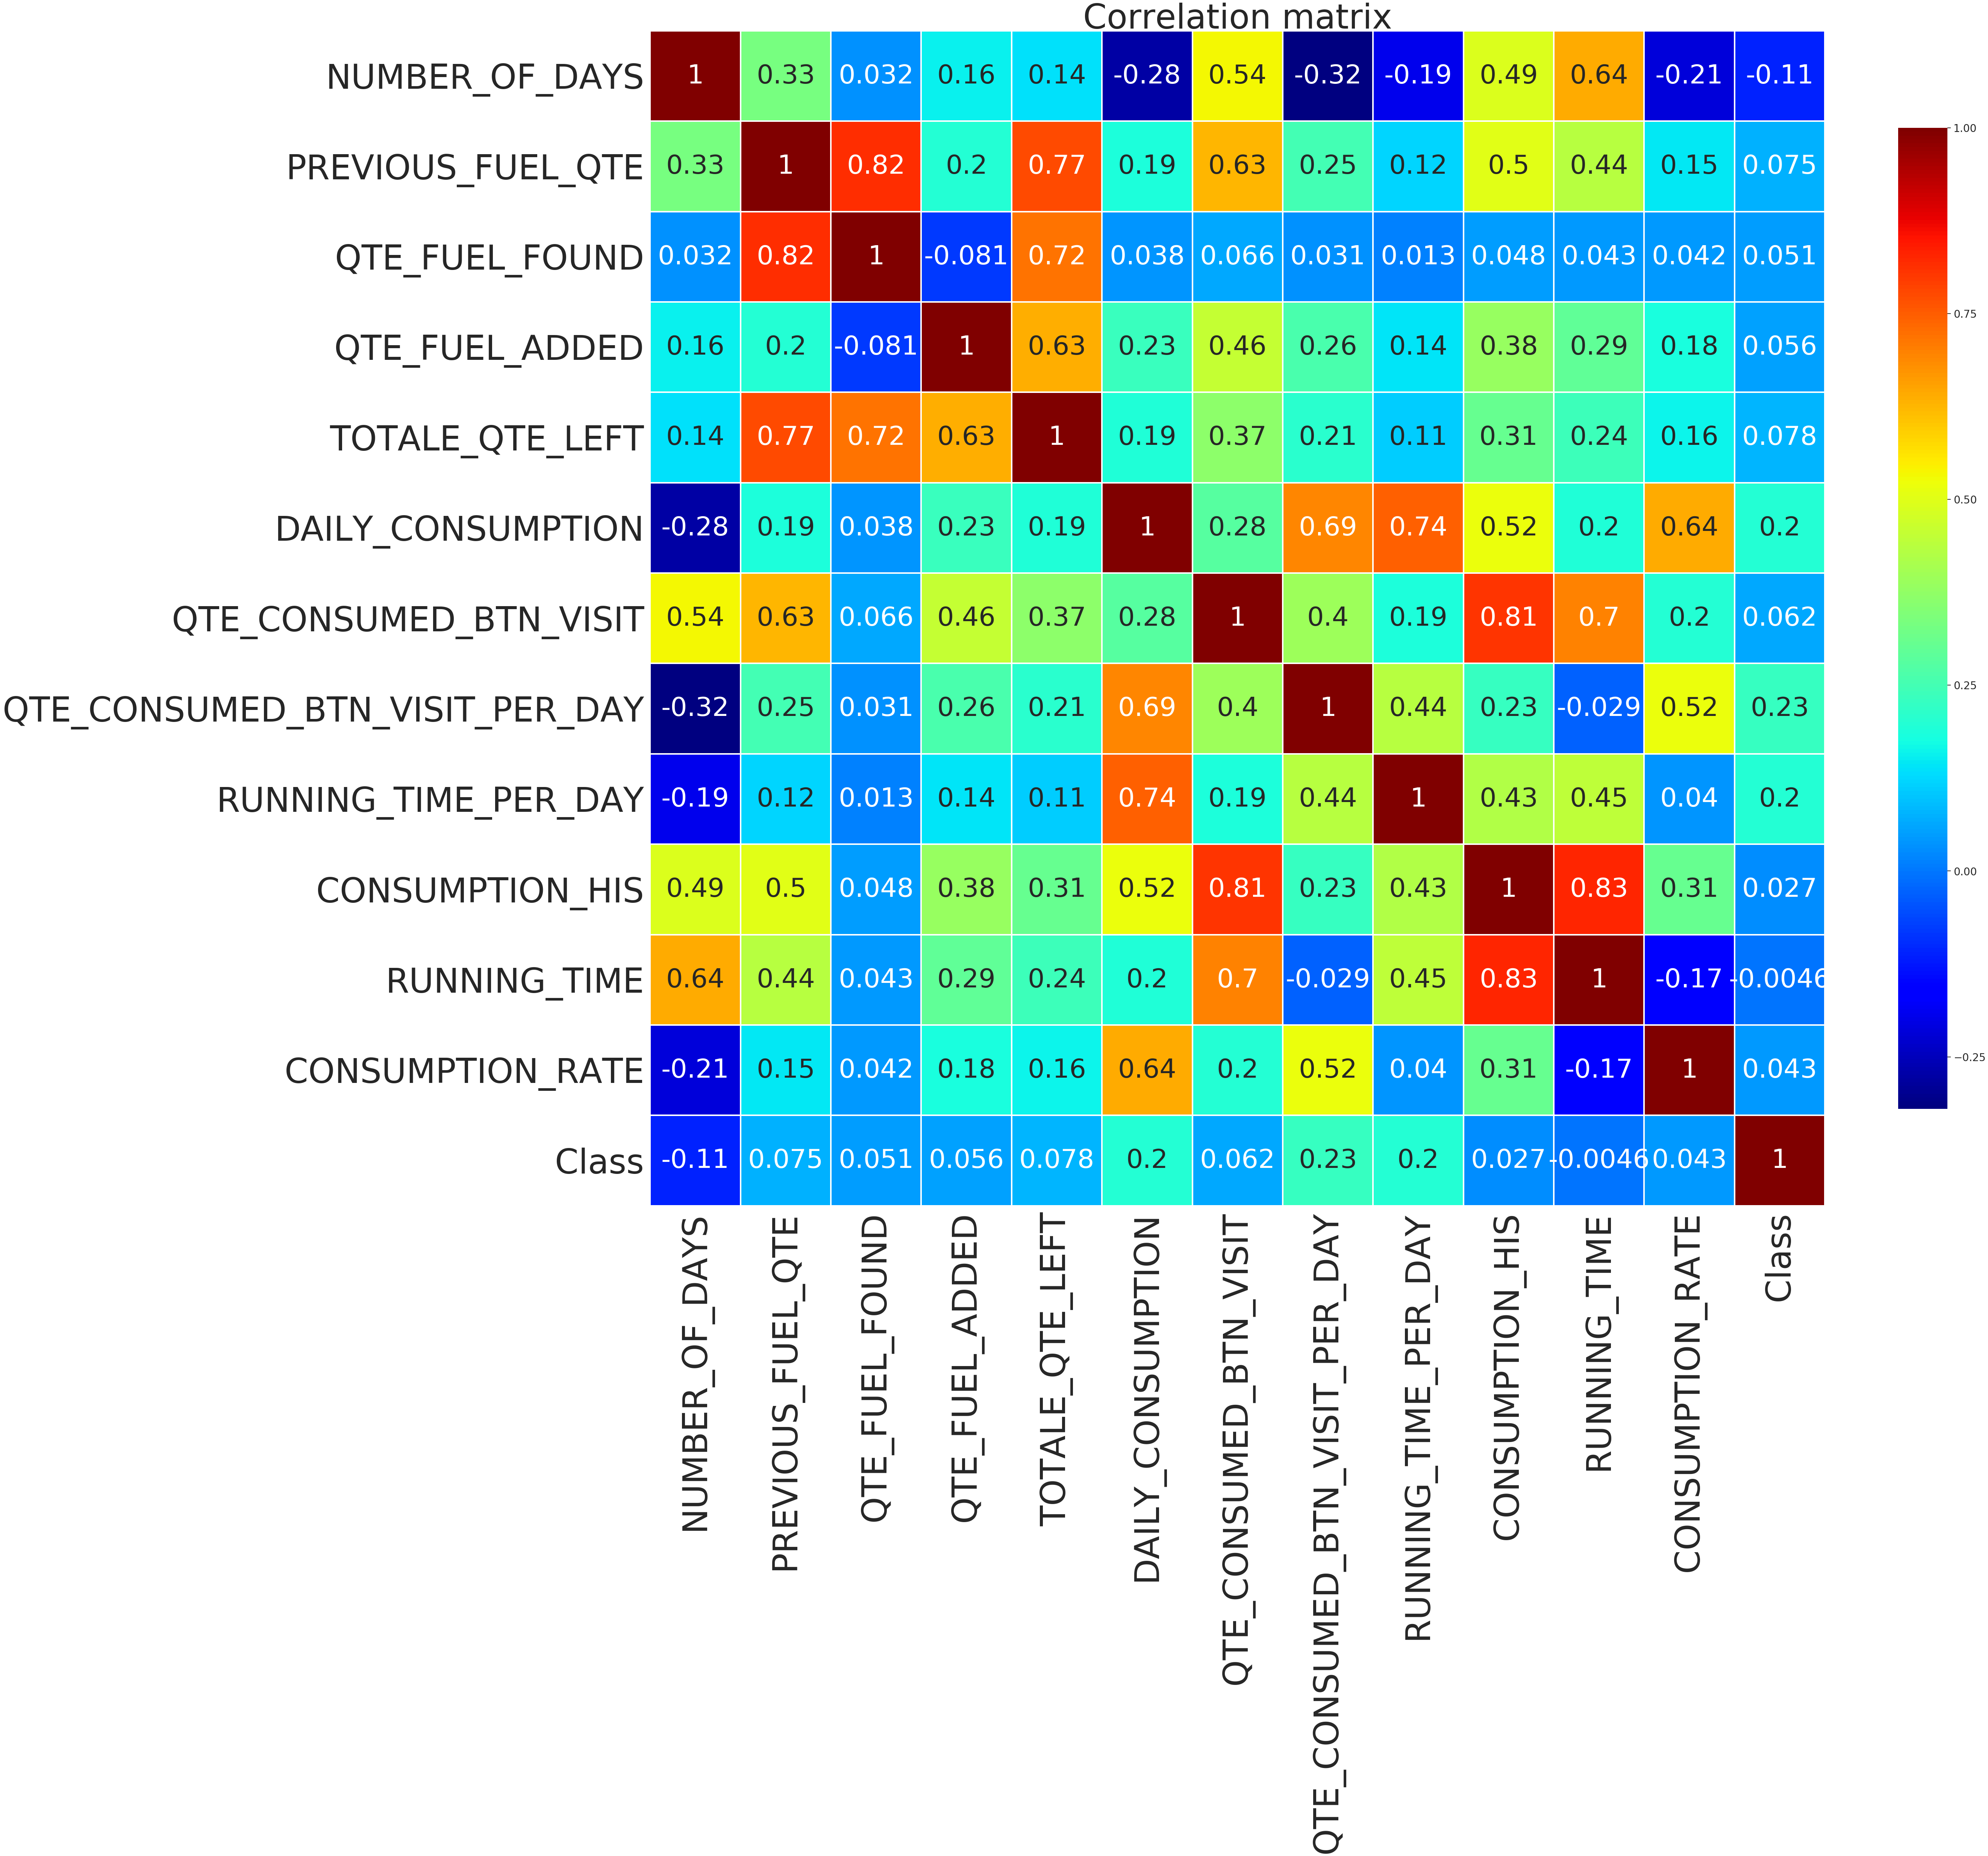
\includegraphics[width=0.9\textwidth]{Figures/correlation_matrix} %
\end{minipage}
	\caption{Correlation Matrix of features}
	\label{fig:correlation matrix}
\end{figure}

The anomalies detected in the data include hours the generator was working in one day, consumption exceeds what fuel generator can consume in one day and the case where generators consume fuel and running time is zero and outliers. The anomalies discovered in the dataset were used to generates a classification class of the samples as either normal or anomaly consumption. 

Figure 	\ref{fig:boxplot} shows the distribution of fuel consumed.
\begin{figure}
	\begin{minipage}[H]{\linewidth}
	\centering
	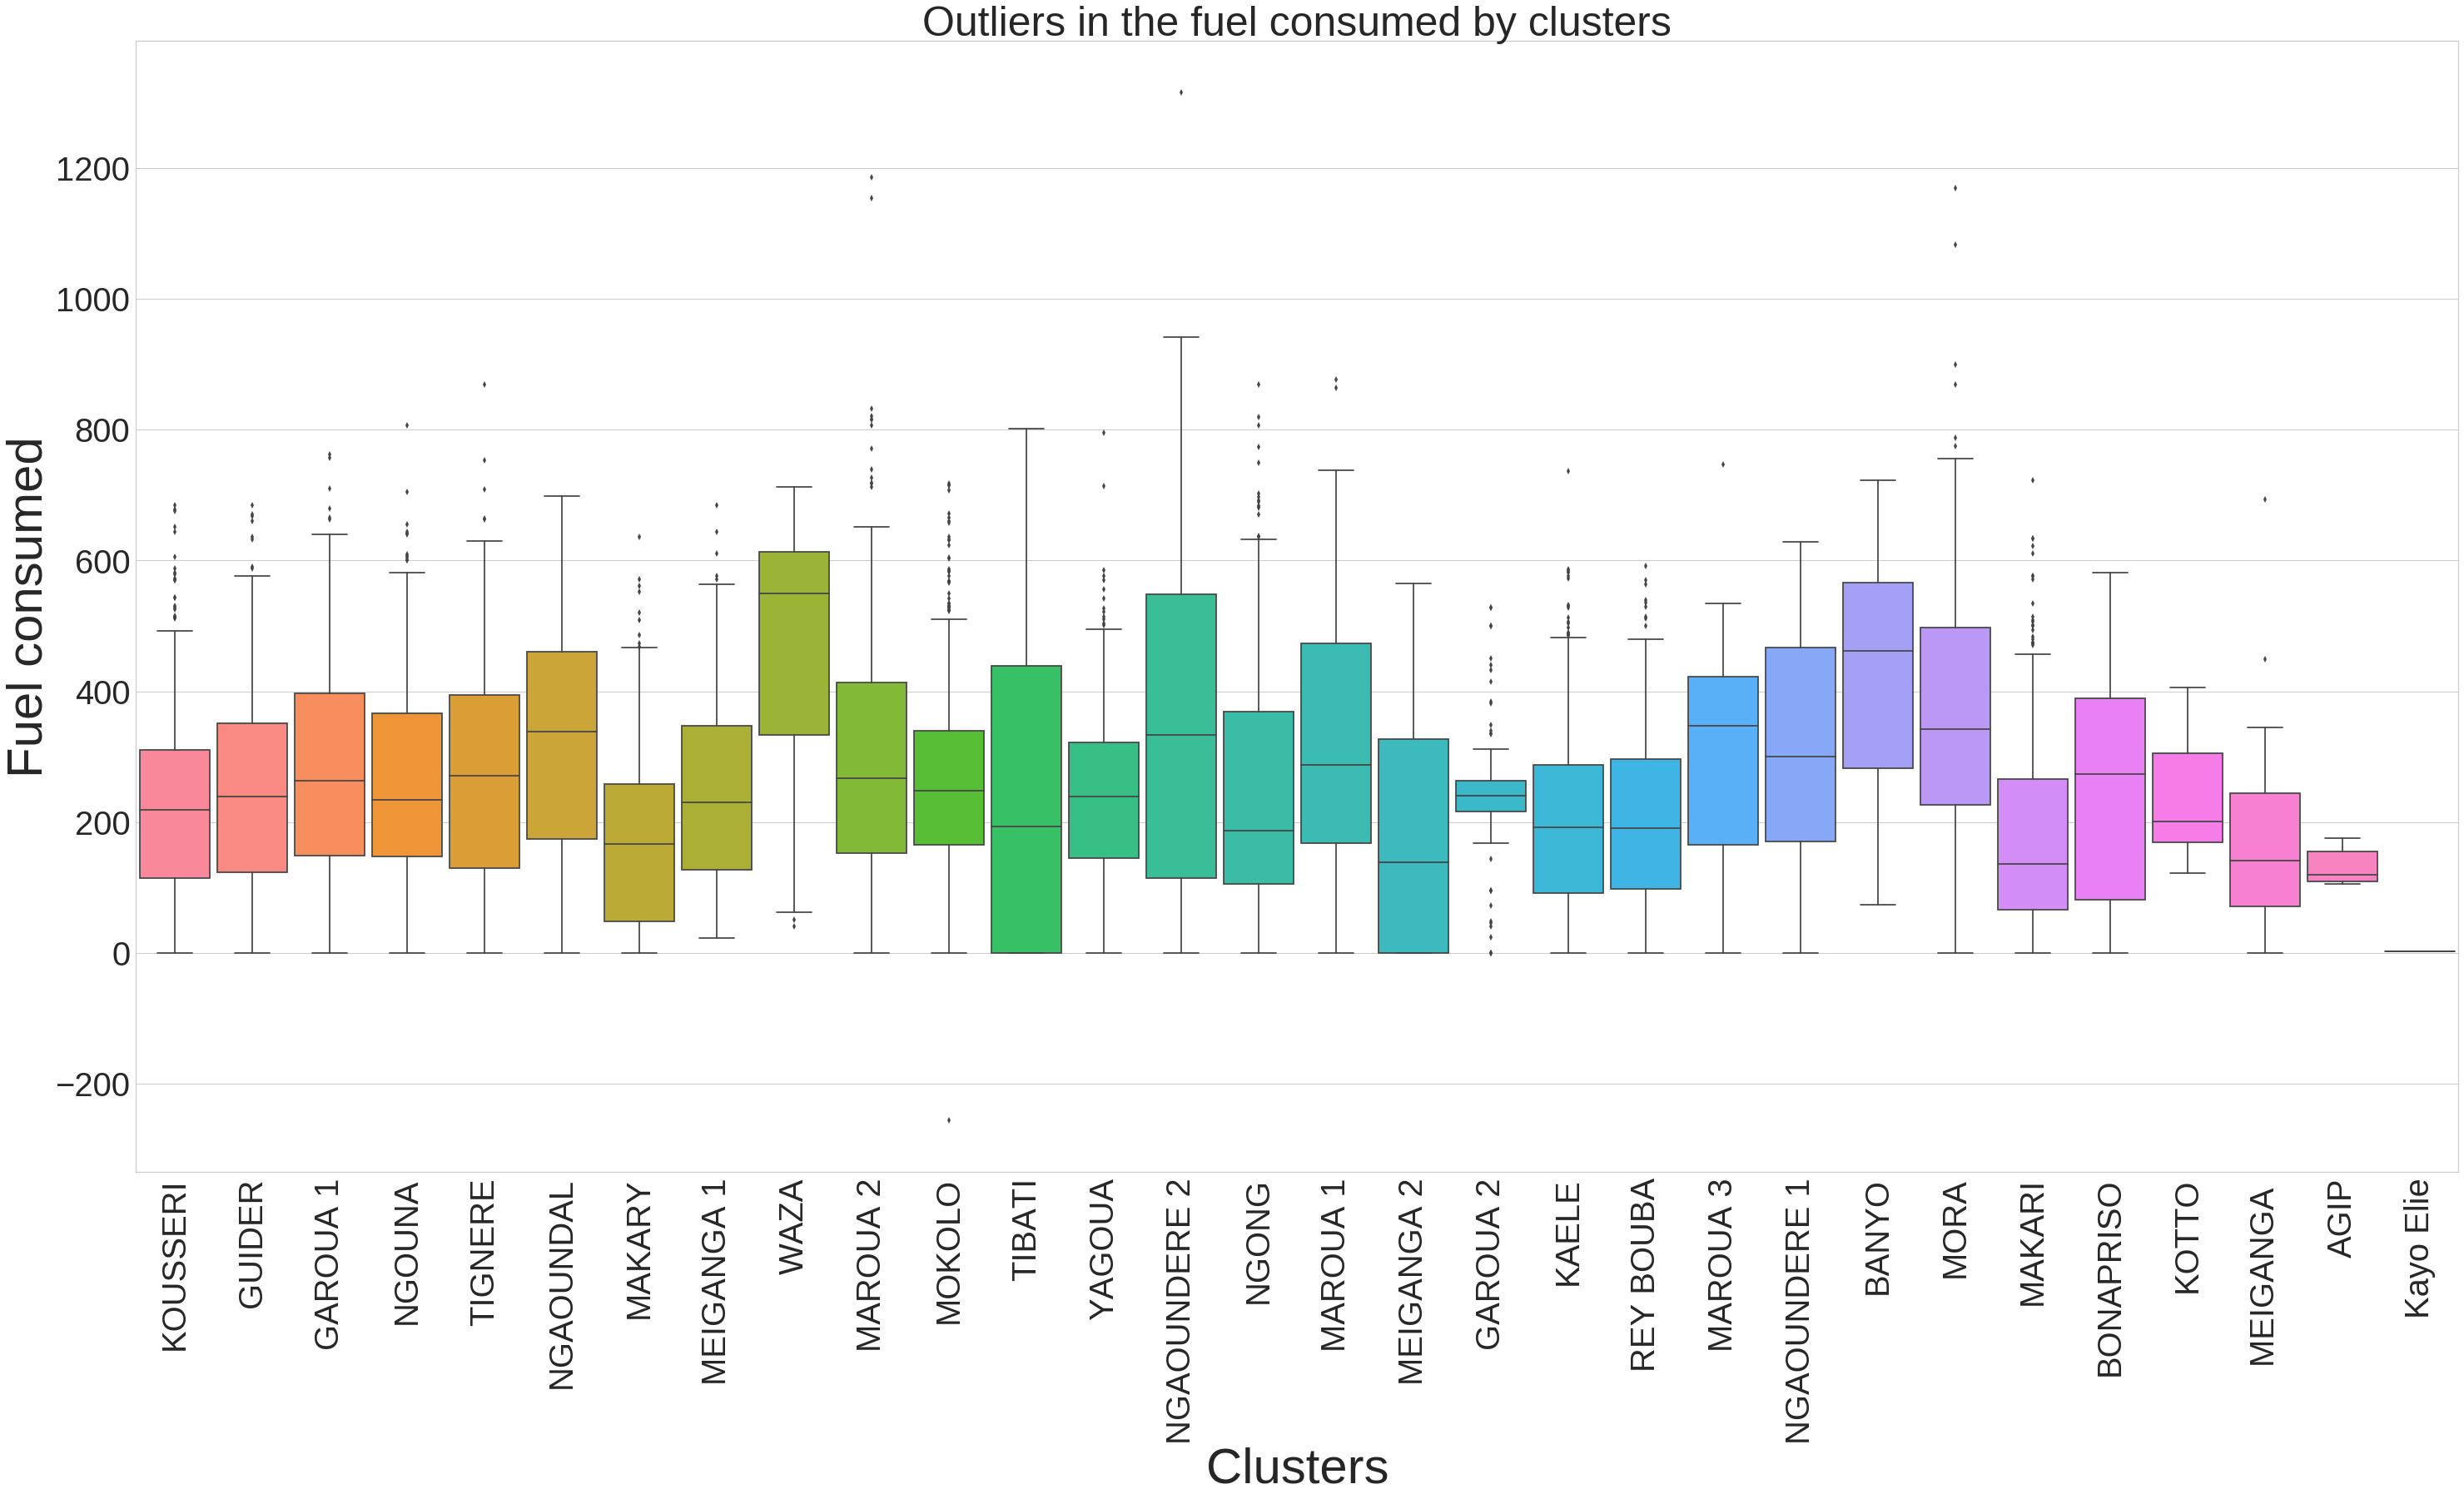
\includegraphics[width=1.1\linewidth]{Figures/Boxplot.png}
\end{minipage}
	\caption{Fuel consumed per cluster.}
	\label{fig:boxplot}
\end{figure}
\mycorrections{Figure \ref{fig:boxplot} shows the fuel consumed by clusters. 
	A cluster is a group of sites where generators are located and each site has a generator and therefore the fuel consumed by a cluster is the total fuel consumed by different generators in various sites}. Clusters show the variation of the fuel consumed with the median of the fuel consumed in most clusters ranges between $200$ and $400$. \mycorrections {To label a sample in the dataset as an anomaly, in this case,  the maximum consumption of each generator was considered and the samples which show the consumptions exceeding the maximum consumption was labeled as an anomaly}. 

The graph \mycorrections { depicted in Figure \ref{fig:rr}} shows a plot of the number hours a generator was working in one day and we observed that the running hours of most of the generator per day fluctuates around $18$ to $25$ hours in a day. \mycorrections{ From the graph, the trend of working hours per day of the generator indicates an abnormal trend with input with more than 24 hours labeled as anomaly}

\begin{figure}
	\begin{minipage}[H]{\linewidth}
	\centering
	\includegraphics[width=1.0\linewidth]{"Figures/Generator"}
\end{minipage}
	\caption{Graph of number of hours the generator function in one day.}
	\label{fig:rr}
\end{figure}

\section{METHODOLOGY} \label{sec:med}
\subsection{Support Vector Machines  }\label{SVM}
Support vector classifier is a supervised machine learning technique used to separate two or more classes by finding a hyperplane which maximizes the margin between them. In the case of linearly separable classes, an ideal hyperplane called decision boundary is defined to separates two classes with the widest margin that ensures the distance between the boundary of the two or more class is maximized \cite{friedman2001elements}. Given a paired of input examples $x\in R $  and corresponding class $d_{i}$ such that  $d_{i} \in \{1, -1\}, $. The classifier find a function that correctly maps each input variable $x_{i}$ to its corresponding class $ d_{i} $.  The decision boundary is defined as;
\begin{equation}\label{eqn4}
f(X) = \textbf{W}^{T}X + b.
\end{equation}
Where $\textbf{W}$ is the weight vector and $b$ the bias. Equation \eqref{eqn4} is a decision boundary determining the class of the input variable. The support vectors, that is, the samples on the boundary of the margin determines the decision boundaries. If $f(X)$  in Equation \eqref{eqn4} is greater than zero then the input variable belongs to class $1$ otherwise it belongs to class $0$. To obtain an ideal hyperplane between the two classes is the same as minimizing the norm of the weight vector \cite{friedman2001elements}. For two-class classification, the input variable is either on the positive or negative side of the decision variable, such that;
\begin{equation}
d_{i}(\textbf{W}^{T}x_{i} + b)\geq 1, \forall (x_{i},d_{i}) \quad , d_{i} \in \{ -1,1\}.
\end{equation}
The margin can be maximized by minimizing the weight vector $\textbf{W}$. In the case of non-separable, penalizing term is introduced to allow misclassification. The slack variable introduced in the case of non-separability measures how far the data deviate from the correct class
\cite{kelleher2015fundamentals}.
\begin{equation}
d_{i}(\textbf{W}^{T}x_{i} + b)\geq 1 - \xi_{i},  \quad i = 1 \cdots N, \quad 0 \leq \xi_{i} \leq 1
\end{equation}
When a sample is correctly classified then the slack variable corresponding to that input value is equal to zero. For non-linear classes, the kernel functions transform the input example to a more separable space. A non-linear kernel function transforms the inputs to a more separable space and defining a hyperplane that clearly separates the classes.  Commonly used non-linear function includes the hyperbolic tangent, polynomial and radial basic kernel \cite{aggarwal2014data}.



\subsection{Multilayer Perceptron }\label{MLP}

MLP is a supervised machine learning neural network inspired \mycorrections{by the human brain \cite{haykin2004comprehensive}}. The classifier consists of input layer, hidden layers, activation function and output layer. The input layer receives the \mycorrections{vector $X = \left[ x_{0}, x_{1},\cdots x_{n}  \right]$ and assigned  weight vector $ w = \left[ w_{0}, w_{1}, \cdots w_{n} \right] $}. MLP is a forward feed, that is,  weighted input variables  move from the input layer to the inner hidden layer \cite{aggarwal2014data}. The hidden layers enhance the model capabilities by allowing the network to learn complex  problem and give result in the output layer. A nonlinear activation function applied to the weighted linear summation of the input variables to extract a relationship between the output and input variable.
\begin{eqnarray}
z  &=& \sum_{i=1}^{m} w_{ji}x_{i},\\
y &= & \phi(z).
\end{eqnarray}
Where $w_{ji}$ is the synaptic weight connecting neurons between the layers and $\phi$ is the activation function which transforms the weighted sum of input.  
The weights vector is unknown, therefore, weights in the input layer are randomly initialized based on the feature importance of the input variables. Hidden layers and activation function allow the model to learn non-linear function, as result, low weight value at the input layer allows the model to start as linear and due to increasing hidden layers,  the model turns nonlinear with increase weights.

Commonly used nonlinear function is the sigmoid function. The weights adjustment is with respect to the error, that is, computed at each neuron to make sure error minimization. As a result of these connections, each node is penalized as every node contributes to the global error computed at the output layer. The aim is to minimize the error, therefore the error correction with respect to the weights  \cite{haykin2004comprehensive}.  \mycorrections {The weight update is done using Gradient descent method given as;}
\begin{equation}\label{enq7}
\Delta w_{ji}^{t} =- \eta\frac{\partial \varepsilon(n)}{\partial w_{ji}}.
\end{equation}
\mycorrections {Where $\eta$ is the learning rate and $\varepsilon(n)$ is the error term. At the output node, the network error is computed. Noting that weights in the hidden layers are updated based on the error computed at the output node.
	Learning rate regulates the change of the adjusted weight in the direction of weight. A small value of $\eta$ controls the step size towards convergence whereas high value will cause divergence.
	To ensure the error is minimized, weights are adjusted such that the new weight became;}
\begin{equation}
w_{kj}^{t +1} =w_{ji}^{t}- \eta\frac{\partial \varepsilon(n)}{\partial w_{ji}}.
\end{equation}
\mycorrections {The weight updates are done either in a batch, that is, using batch gradient descent or is the stochastic gradient descent method.}
\subsection{K- Nearest Neighbor }
\mycorrections{We also made use of KNN classifier to perform anomaly detection. }
KNN is a lazy learning algorithm that depends on the knowledge gained from the training data to predict the test data. The algorithm does not make any assumptions about the data and base its prediction according to the   $k$ neighboring terms. The $k$ neighbors parameter that determined the number of neighbors in the training dataset to consider. To predict the class of test data point, Euclidean or Manhattan distance is applied in the case of the continuous variable. The commonly used distance is the Euclidean as it can be used for both nominal and numerical variable and distance is easy to interpret. Euclidean distance is measured by taking the difference between features in the data point i.e;
\begin{equation}
D = || x_{j} - x_{0} ||.
\end{equation}

\mycorrections { Since KNN  depends on the number of neighbors $k$ during its testing phase and the algorithm uses distance measure to determine test class, the algorithm suffers from high computation cost.  The choice of the value $k$ influences the performance of the model. A small value of $k$ can result in high accuracy but can results in overfitting the model whereas for a large value of $k$, although the effect of noise is reduced, KNN is prompt to have lose boundary hence underfitting the model. }
\subsection{Logistic Regression }
\mycorrections {Logistic regression makes use of conditional probability to map the input variable to a corresponding classification class. Given an input variable, the model predicts the probability of an input variable to belong to classification class}. Suppose given an input variable $X$ such that , $X = \left[ x_{0} , x_{1},\cdots x_{n}\right]$, and the corresponding class $Y_{i}, \forall i = 1,\cdots,P $. Where P represents the number of class, LR uses non-linear activation, that is, the sigmoid function to give the relation between the input variables and the output class. In this case of binary classification such that, Y $ \in \{ 0,1\}$ with a probability of being in either class 1 or 0 is given by;
\begin{equation}
p(Y| X) = \frac{1}{ 1 + e^{-z}}, \quad z = w_{0} + \sum_{i = 1}^{n} W^{T}X
\end{equation}

The aim of logistic regression is to optimize the weights parameters $\textbf{W}$ such that the classification error is minimized. Parameters are estimated by either gradient ascent or stochastic gradient ascent method \cite{bonaccorso2017machine}. The log-likelihood and Newton methods are commonly applied to find optimal parameters \cite{qi1993nonsmooth}. In both gradient ascent or stochastic gradient ascent method, parameters are adjusted until the model has a minimum error between the observed value and the predicted. Stochastic gradient ascent updates its weight at every single point depending on the direction of the weight.

The gradient ascent  differs from the stochastic gradient ascent method in the sense that weights are adjusted at every level of the input variable and the gradient ascent considers  input dataset in batches at each step, that is, to optimize the parameters using gradient ascent the problem is solved by  taking the partial derivate of log-likelihood  function with respect to parameters. 


\subsection{Performance evaluation}
To evaluate the predictive capabilities performance of the fitted models, we abort methods such as train-test split and K-fold cross validation methods.  From prediction of the test data, the model prediction was evaluated using confusion matrix. Table \ref{tab} shows the representation of a binary classification in a confusion matrix. 
%The dataset was split with $80\% $ for training set and $20\%$ test set. The testing sample validates the performance of the model in the confusion matrix and the generalized score of the model is obtained. The classifiers are trained on the same dataset and the performance is evaluated using the test dataset. The confusion matrix is a  matrix that shows the classifier ability to predict the test data. Below is a representation of Confusion matrix used to decide the different performance of classifiers. 


\begin{tabular}{c|c|c|c|c}
	
	\multicolumn{2}{c}{}&\multicolumn{2}{c}{}&\\
	\cline{3-4}
	\multicolumn{2}{c|}{}&Positive&Negative&\multicolumn{1}{c}{}\\
	\cline{2-4}
	\multirow{2}{*}{}& Positive & True Positive (TP) &False Positive (FP) & \\
	\cline{2-4}
	& Negative & False Negative (FN) & True Negative (TN) & \\
	\cline{2-4}
	
\end{tabular}
\captionsetup{type=table} 
\caption{Confusion Matrix }
\label{tab}


From Table \ref{tab}, the following information about the classifier's performances can be obtained.\\

True positive (TP): correct prediction of positive class

True negative (TN): predictions of negative class when the class is actually negative 

False negative (FN): wrong prediction of positive class as negative.

False positive (FP): model predicts negative class predicted as positive.

% From the confusion matrix, the True positive rate (TPR) is obtained by diving the true positive predicted by the total number of positive in the sample and the False positive rate (FPR) derived from the division of the false positive and the total number of negative in the sample. 

Recall or sensitivity gives the classifier capability to correctly classify the positive class which is given as a ratio of TP and positive in the sample in the dataset. Other measures such as precision compare the true positive in the confusion matrix and the total number of positively predicted by the classifier. Specificity is also known as the true negative rate of the classifier, it is the ratio of true negative and negatives sample. F-measure the Harmonic mean of recall and precision. Equation \eqref{q1} to \eqref{q2} gives the  formulas of the  computation generated from the confusion matrix 

\begin{equation}\label{q1}
Accuracy = \frac{TP +TN}{TP +FP +TN+FN} .
\end{equation}
\begin{equation}\label{eqn11}
Recall(Sensitivity) = \frac{TP }{TP +FN}. 
\end{equation}
\begin{equation}\label{eqn12}
Precision = \frac{TP}{TP +FP}.
\end{equation}
\begin{equation}
F-measure = 2\frac{Precision*Recall}{Precision +Recall}.
\end{equation}
\begin{equation}\label{q2}
Specificity (TNR) = \frac{TN}{TN +FP}.
\end{equation}
For ease of comparison, models from all techniques in our study were developed using the same derived attributes.\\

Cross validation is a technique used to check how the model will perform in general. We performed K-fold cross-validation with $10$ fold. The data are split into K folds, that is, $10$ folds, nine folds are used to train the data and the tenth fold is used for testing, this process is repeated until all the folds are trained and tested. The accuracy of the classifier is obtained by taking the average of all accuracy obtained in the test fold. 

Due to the imbalanced nature of the normal and anomaly class in our dataset, ROC curves were used to measure how classifier is doing in each class. As we saw earlier, the data is skewed and therefore class distribution might affect classifier performance. The area under the curve (AUC) visualize the classifier behavior on how often the model will classify positive class correctly and when the actual classification is negative how often the model predicts positive. We want to maximize the true positive rate and minimize the false positive rate. The curve has TPR on the vertical axis and FPR on the horizontal axis. The plot range from  $0 -1$ with position (0,1) indicates a perfect classification model.  
The TPR and the FPR of the classifier is given by;
\begin{equation}
TPR = \frac{TP }{TP +FN}.
\end{equation}
\begin{equation}\label{q19}
FPR = \frac{FP}{FP +TN}.
\end{equation}
ROC curve has better visualization of models performance and comparative analysis of classifiers \cite{japkowicz2011evaluating}.  The precision-recall curve is more appropriate to study the behavior of the classifier. Precision and recall of a classifier is given by  Equation  \eqref{eqn12} and \eqref{eqn11}. The precision-recall curve gives a clear relation of a true positive classified sampled and false positive classified sampled. The relationship between precision-recall and ROC curve shows that there exists a one-to-one relationship between the two curves \cite{davis2006relationship}. If the curve of classifier dominates the area under the curve in the precision-recall curve then curve must also dominate the ROC curve.

\section{RESULTS \& ANALYSIS} \label{sec:resu}
In this section, we are discussing the ability of the model to correctly predict the test dataset. Classification techniques were fitted with real-life data with $80\%$ as a training sample and $20\%$ for testing. To conduct a comparison of the fitted models, we compared the performance of the classifiers on the test data term of accuracy, graphical evaluation techniques such as ROC and precision-recall curve and K-fold cross validation technique. Anomalies detection abilities of the algorithms were also studied, that is, to identify which algorithm correctly predicts the two classes with minimal classification error. SVM, KNN, and MLP show an impressive result in identifying the anomalies in the data. Table \ref{tab4} shows the confusion matrix results of the classifiers on test data of $1181$ sample points.
\begin{center}
	\begin{tabular}{ |p{0.7cm}|p{0.7cm}|p{0.7cm}|p{0.7cm}|p{0.7cm}|} 
		\hline
		\hline
		\multicolumn{5}{c}{\cellcolor{gray!50}Confusion matrix} \\
		\hline
		\hline
		\cline{1-5}
		
		&SVM&MLP&KNN&LR \\
		& && & \\
		& && & \\
		\cline{1-5}
		TR &752&773&696 &741   \\
		\hline
		FP&  30   &9&86&41	\\
		\hline
		TN&369&362	&310&95	\\
		\hline
		FN &30& 37&89&304	\\
		\hline
	\end{tabular}
	\caption{Classifier confusion matrix }
	\label{tab4}
\end{center}
The  summary of classifiers performance on the evaluation metrics used in this study are shown in  Table \ref{tab2}. 
\begin{center}\label{kk}
	\begin{tabular}{ |p{1.1cm}|p{1.0cm}|p{1.1cm}|p{1.0cm}| p{1.1cm}|p{1.3cm}|} 
		
		\hline
		\multicolumn{6}{c}{\cellcolor{gray!50}Classification performance } \\
		\hline
		\hline
		\cline{1-6}
		
		&Accuracy &F1-Measure & Recall& Precision& Specificity\\
		Classifier & & & & &\\
		\cline{1-6}
		LR &0.708& 0.811&  	0.709 &0.943&0.699\\
		\hline
		SVM&   0.949  &0.962&	0.962 &0.962&0.925\\
		\hline
		KNN&0.851 &	0.888 &	0.887&0.890&0.783\\
		\hline
		MLP & 0.961& 0.971&	0.954&0.988&0.976 \\
		\hline
	\end{tabular}
	%	\caption{Classifier evaluation performance }
	\label{tab2}
\end{center}

SVM  fitted with radial basis function (RBF) had a general score of $94.9\%$ on the test data.  Although, the SVM had higher accuracy compared to KNN and LR on the test it is outperformed by MLP. From results obtained in the 10-fold cross validation as shown in Figure \ref{fig:k-foldcrossvalidation}, SVM had an average score of $95.3\%$. The ROC and precision-recall curve of SVM as from Figure \ref{fig:rocall} shows that SVM has an AUC of $0.96$ and $ 0.98\%$ in precision-recall curve and ROC curve respectively.

\begin{figure}
	\centering
	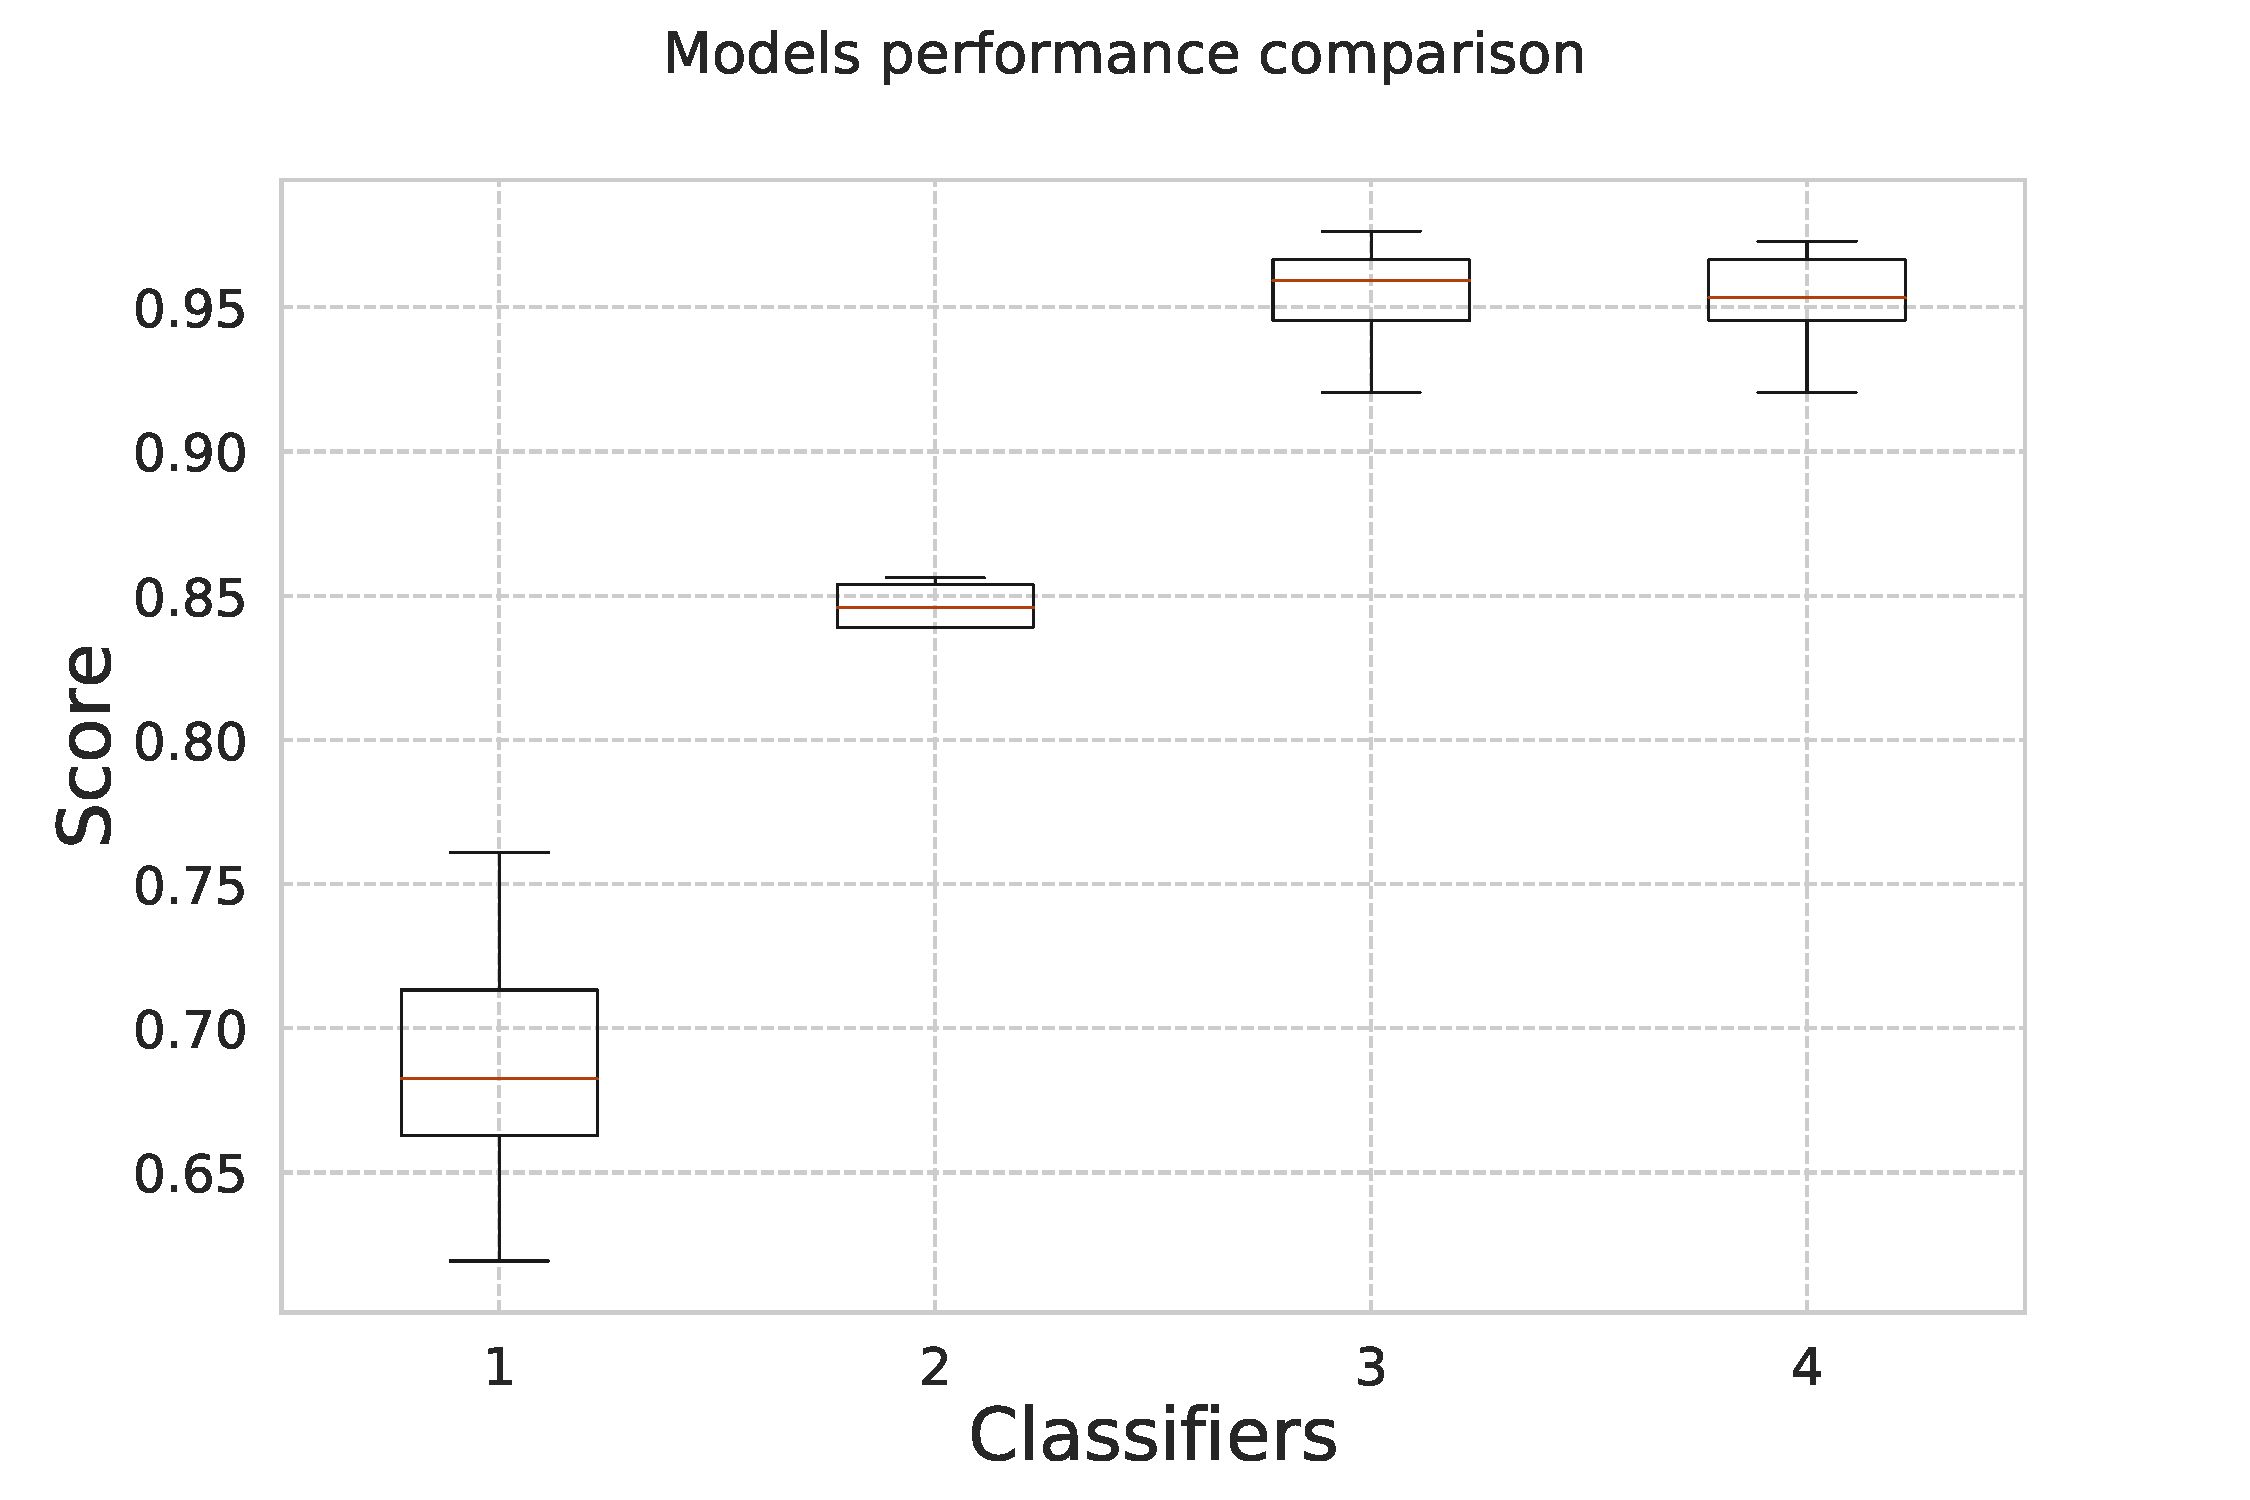
\includegraphics[width=0.7\linewidth]{Figures/K-fold_cross_validation.pdf}
	\caption{10-Fold cross validation score for LR, KNN, MLP, and SVM}
	\label{fig:k-foldcrossvalidation}
\end{figure}

MLP fitted with relu activation shows better performance compared to other classifiers. The input variable used to fit the model were all standardized to ensure the feature are equally treated in the regularization. From the  10-fold cross validation, the classifier had an average score of $95.5\%$. As shown from Figure \ref{fig:rocall}, the classier had an AUC of $1.00$ and $0.99$ for the ROC and precision-recall curves respectively. The precision-recall curve of MLP dominates with a score closed to perfect performances as compared to other classifiers.  

KNN fitted with $k$ equals to three had a general score of $85.1\%$ on the prediction of the test data. For the case of anomalies detection, KNN performed better as compared to LR. From the 10-fold cross validation score, the KNN has a score of $84.3\%$, which outperformed LR. From Figure \ref{fig:rocall}, KNN had an AUC of $0.89$ and $0.96$ in ROC and precision-recall curve respectively. 

LR fitted with parameter  C equal to $10$. The classifier had a general performance of $70.8\%$ on the test data and $69\%$ K-fold cross validation score with ten fold. From Table \ref{tab4}, the classifier identified normal class with a precision of $94.3\%$ which is slightly better as compared to KNN, and recall of LR indicates  $70.9\% $. From Figure \ref{fig:rocall},  AUC of ROC curve in LR is close to the random guess with an AUC of $69\%$ in the ROC curve. In this case, the classifier will randomly classifier a sample, hence low predictive performance. LR had the lowest predictive performance in identifying the anomaly class.
%\begin{center}
%	\begin{tabular}{ |p{1.2cm}|p{1.2cm}|p{1.2cm}|p{1.2cm}|p{1.2cm}|} 
%		\hline
%		0

Across all validation tests, the LR is under performing In the study, accuracy techniques were used to determine the performance. Comparing the performance of the models, MLP has best accuracy score of $96.1\%$ on test data. SVM, KNN, and LR had an accuracy score of $94.9\%$, $85.1\%$ and $70.8\%$ respectively. From figure \ref{fig:rocall}, ROC and precision-recall curve of MLP compared to other classifier. 

Figure \ref{fig:rocall} shows the precision-recall and ROC curves representation of the classifiers used in this study. Precision-recall curve evaluates the number of positives that the model predicted. The curve at the right corner of the precision-recall curve is considered to have more true positive predicted by the model as compared to false negative. Precision-recall curve focus on how much positive have been predicted correctly given the total positive predicted. The  precision-recall curve of LR have a drastic change, this is explained by the change of positive and negative samples predicted as shown in Table \ref{tab4}. The graphs below show the graphical evaluation measure of the classifiers using precision-recall and ROC curves.  
\begin{figure}
	\begin{minipage}[H]{\linewidth}
	\centering
	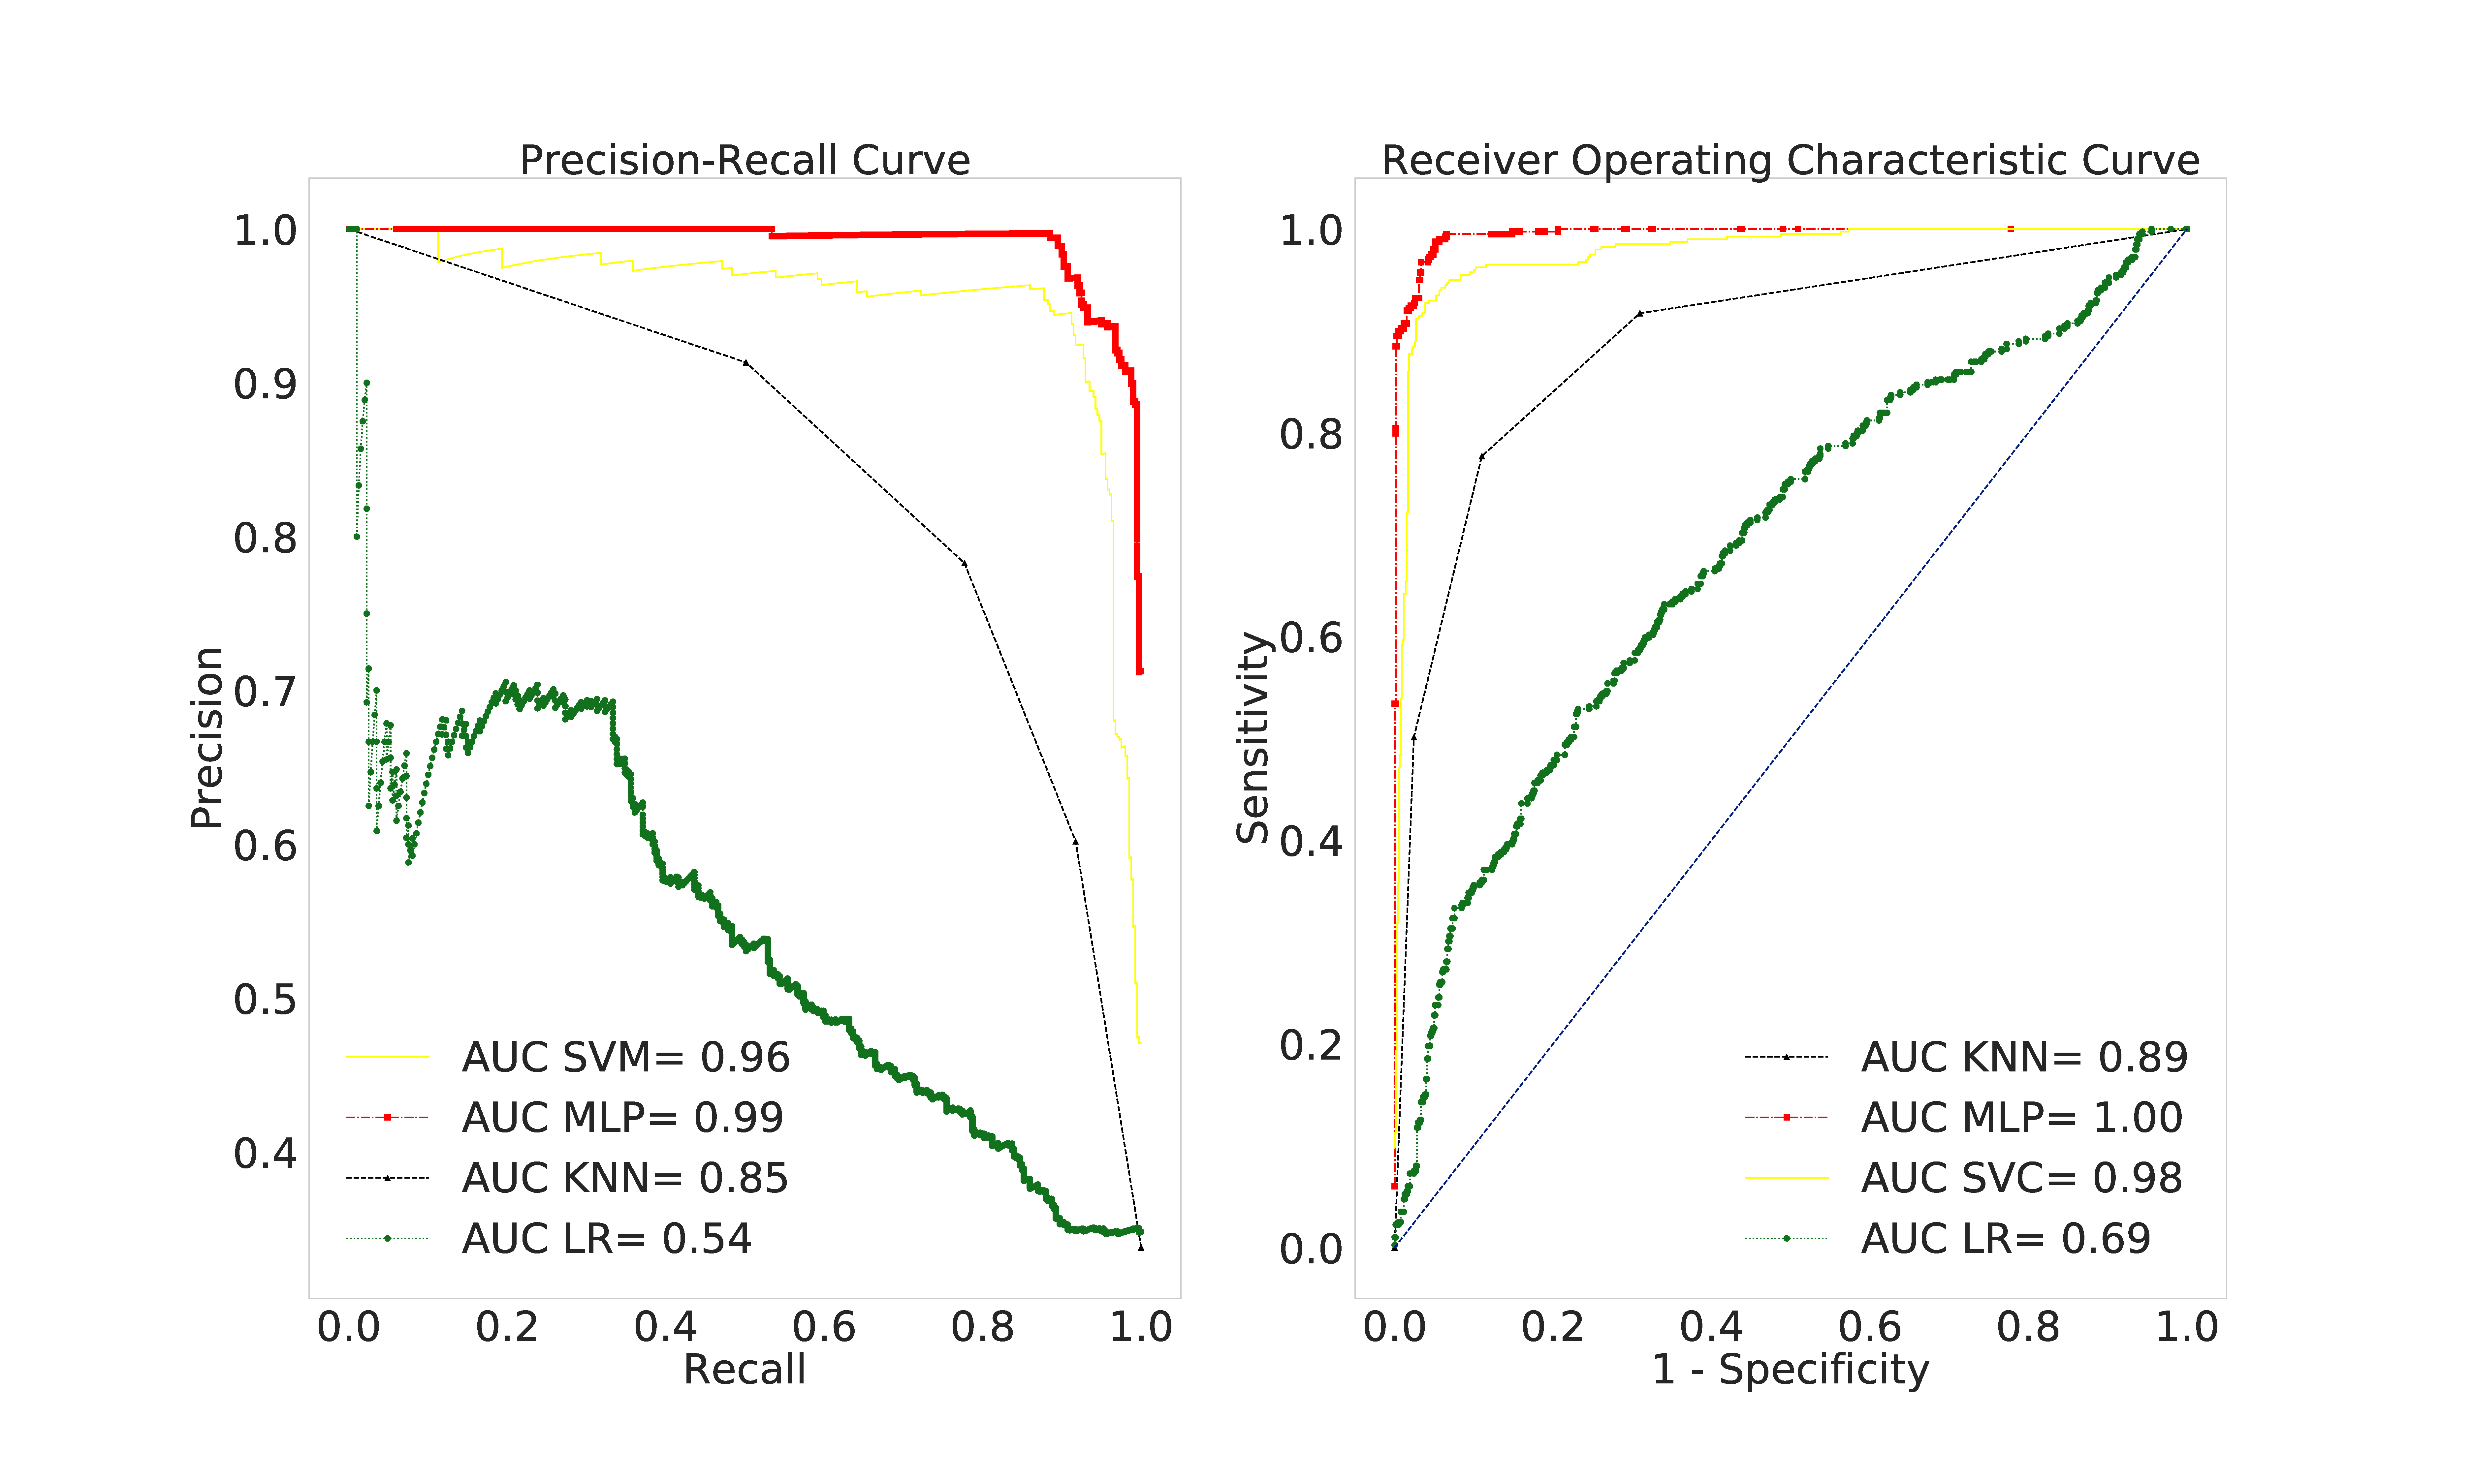
\includegraphics[width=1.1\linewidth]{Figures/ROC&PR.pdf}
\end{minipage}
	\caption{\textit{Precision-Recall curves and ROC curves of classifiers} }
	\label{fig:rocall}
\end{figure}

\subsection{Bias-Variance analysis}
Using cross validation with ten split, we observe the relationship between training score and cross validation score of different classifiers. Variation of cross validation curve is as a result of high variance and training score curve variation is as a result of high bias. Bias-variance in the model affects the performance of the model. High variance is an indication that the model learns every noise in the data. High bias indicates that the model has less information about the dataset. Regularization of bias and variance help the model to attain better predictive performance. \\

From cross validation with ten fold, Figure \ref{fig:crossval} shows the cross validation and the training scores on the fitted dataset.\\

\begin{figure*}
	\begin{minipage}[H]{\linewidth}
	\centering
	\includegraphics[width=0.7\linewidth]{Figures/learning}
\end{minipage}
	\caption{Training and cross validation score curve of MLP, KNN, SVM, and LR}
	\label{fig:crossval}
\end{figure*}
In all the models the cross validation curve tends to converge with increasing training sample although SVM  and KNN the convergences is slow with increasing in the sample.  The training and cross validation curve of MLP from Figure \ref{fig:crossval} convergence faster and therefore increase in training data does not improve its performance. In LR, training score and cross validation curves converge completely with an increase in the data examples.
\pagebreak
\section{CONCLUSION}

In this paper, we aimed at evaluating the classification algorithm by training the model to learn and identify the anomalies in the fuel consumed dataset from a telecommunication base station. Four classification techniques were evaluated namely, SVM, LR, MLP, and KNN. MLP had the best performance generally with an accuracy score on the test data of $96.1\%$. Although SVM outperformed other classifiers such as KNN and LR, using K- fold cross validation technique MLP performed best with a score of $96.1\%$. From the confusion matrix, MLP had the best predicting power of the anomalies. LR performed better in the precision score as compared to KNN, the classifier had the lowest performance as compared to all the classifiers. LR predicts more of the normal class as compared to anomaly class. The dataset was imbalance and as a result, evaluation methods which depend on both class for computation provides wrong impression due to skew nature of the class.  ROC and Precision-recall curve used to visualize and evaluates classifiers. From Figure \ref{fig:rocall}, MLP dominates two graphs with higher performance on AUC in both curves. 
For anomalies detection in the dataset, MLP had the highest performance. The anomaly is our class of interest and since the ROC curve takes into consideration of the negative class, ROC curve became the most relevant graphical visualization measure for not only the study of classifier behavior but also for model selection through a comparative evaluation of different classifiers. We, therefore, conclude MLP show an overall better performance compared to other classification techniques in the performance measures, that is, the classifier best fit the training examples compared to other classifiers in terms of anomaly detection and in evaluation performance such as K-fold cross validation, train-test split, precision-recall, and ROC curves.  




\section{SUMMARY}
We fitted SVM, MLP, LR, and KNN on the dataset of fuel consumed by the generator with two class, anomaly and normal class. Comparative analysis of classifiers performance using K-fold cross validation, train test spit, graphical representation techniques such as ROC and precision-recall curve were used to study the behavior of the classifier. Key indicating factors consider to evaluate the classifiers includes how well the classifier identify anomalies that exist in the test data, accuracy and AUC in ROC graph. From the results of this study, MLP performed well in all metrics evaluated. The distribution of the two-class was not equal, therefore the classification accuracy was less considered in the model selection. 

\section{Acknowledgement }
The author would like to thank TeleInfra Company and Group One Holding Company for providing the dataset for this study. We wish to acknowledge Mr. OKALI DIMA Patrick from Group one holding for ensuring the data was available. Grateful for SciKit \footnote{{\tt https://scikit-learn.org/stable/modules/generated/sklearn.svm.SVC.html}} learn library as this work has been made possible from the use of their library packages.
\section{References} \label{sec:references}
\bibliographystyle{elsarticle-harv} 
\bibliography{ref.bib} %{<your bibdatabase>}
%% else use the following coding to input the bibitems directly in the
%% TeX file.
% \begin{thebibliography}{00}
% 
% %% \bibitem[Author(year)]{label}
% %% Text of bibliographic item
% 
% \bibitem[ ()]{}
% 
% \end{thebibliography}

%%
%% End of file `elsarticle-template-harv.tex'.
%
%\begin{enumerate}[(1)]
%\item Group the authors per affiliation.
%\item Use footnotes to indicate the affiliations.
%\end{enumerate}
%See the front matter of this document for examples. 
%You are recommended to conform your choice to the journal you 
%are submitting to.
%
%\section{Bibliography styles}
%
%There are various bibliography styles available. You can select the
%style of your choice in the preamble of this document. These styles are
%Elsevier styles based on standard styles like Harvard and Vancouver.
%Please use Bib\TeX\ to generate your bibliography and include DOIs
%whenever available.
%
%Here are two sample references: 
%\cite{XUDONG:1999}
%\cite{XUDONG:1999,FAN:1999}
%\cite{XUDONG:1999,MIYAZAKI:2000}
%
%\section{Floats}
%{Figures} may be included using the command,\linebreak 
%\verb+\includegraphics+ in
%combination with or without its several options to further control
%graphic. \verb+\includegraphics+ is provided by {graphic[s,x].sty}
%which is part of any standard \LaTeX{} distribution.
%{graphicx.sty} is loaded by default. \LaTeX{} accepts figures in
%the postscript format while pdf\LaTeX{} accepts {*.pdf},
%{*.mps} (metapost), {*.jpg} and {*.png} formats. 
%pdf\LaTeX{} does not accept graphic files in the postscript format. 
%
%\begin{figure}
%	\centering
%		
\includegraphics[scale=.75]{Fig1.pdf}
%	\caption{The evanescent light - $1S$ quadrupole coupling
%	($g_{1,l}$) scaled to the bulk exciton-photon coupling
%	($g_{1,2}$). The size parameter $kr_{0}$ is denoted as $x$ and
%	the \PMS is placed directly on the cuprous oxide sample ($\delta
%	r=0$, See also Table \protect\ref{tbl1}).}
%	\label{FIG:1}
%\end{figure}
%
%
%The \verb+table+ environment is handy for marking up tabular
%material. If users want to use {multirow.sty},
%{array.sty}, etc., to fine control/enhance the tables, they
%are welcome to load any package of their choice and
%{cas-dc.cls} will work in combination with all loaded
%packages.
%
%\begin{table}[width=.9\linewidth,cols=4,pos=h]
%\caption{This is a test caption. This is a test caption. This is a test
%caption. This is a test caption.}\label{tbl1}
%\begin{tabular*}{\tblwidth}{@{} LLLL@{} }
%\toprule
%Col 1 & Col 2 & Col 3 & Col4\\
%\midrule
%12345 & 12345 & 123 & 12345 \\
%12345 & 12345 & 123 & 12345 \\
%12345 & 12345 & 123 & 12345 \\
%12345 & 12345 & 123 & 12345 \\
%12345 & 12345 & 123 & 12345 \\
%\bottomrule
%\end{tabular*}
%\end{table}
%
%\section[Theorem and ...]{Theorem and theorem like environments}
%
%{cas-dc.cls} provides a few shortcuts to format theorems and
%theorem-like environments with ease. In all commands the options that
%are used with the \verb+\newtheorem+ command will work exactly in the same
%manner. {cas-dc.cls} provides three commands to format theorem or
%theorem-like environments: 
%
%\begin{verbatim}
% \newtheorem{theorem}{Theorem}
% \newtheorem{lemma}[theorem]{Lemma}
% \newdefinition{rmk}{Remark}
% \newproof{pf}{Proof}
% \newproof{pot}{Proof of Theorem \ref{thm2}}
%\end{verbatim}
%
%
%The \verb+\newtheorem+ command formats a
%theorem in \LaTeX's default style with italicized font, bold font
%for theorem heading and theorem number at the right hand side of the
%theorem heading.  It also optionally accepts an argument which
%will be printed as an extra heading in parentheses. 
%
%\begin{verbatim}
%  \begin{theorem} 
%   For system (8), consensus can be achieved with 
%   $\|T_{\omega z}$ ...
%     \begin{eqnarray}\label{10}
%     ....
%     \end{eqnarray}
%  \end{theorem}
%\end{verbatim}  
%
%
%\newtheorem{theorem}{Theorem}
%
%\begin{theorem}
%For system (8), consensus can be achieved with 
%$\|T_{\omega z}$ ...
%\begin{eqnarray}\label{10}
%....
%\end{eqnarray}
%\end{theorem}
%
%The \verb+\newdefinition+ command is the same in
%all respects as its \verb+\newtheorem+ counterpart except that
%the font shape is roman instead of italic.  Both
%\verb+\newdefinition+ and \verb+\newtheorem+ commands
%automatically define counters for the environments defined.
%
%The \verb+\newproof+ command defines proof environments with
%upright font shape.  No counters are defined. 
%
%
%\section[Enumerated ...]{Enumerated and Itemized Lists}
%{cas-dc.cls} provides an extended list processing macros
%which makes the usage a bit more user friendly than the default
%\LaTeX{} list macros.   With an optional argument to the
%\verb+\begin{enumerate}+ command, you can change the list counter
%type and its attributes.
%
%\begin{verbatim}
% \begin{enumerate}[1.]
% \item The enumerate environment starts with an optional
%   argument `1.', so that the item counter will be suffixed
%   by a period.
% \item You can use `a)' for alphabetical counter and '(i)' 
%  for roman counter.
%  \begin{enumerate}[a)]
%    \item Another level of list with alphabetical counter.
%    \item One more item before we start another.
%\end{verbatim}
%
%Further, the enhanced list environment allows one to prefix a
%string like `step' to all the item numbers.  
%
%%\pagebreak
%\begin{verbatim}
% \begin{enumerate}[Step 1.]
%  \item This is the first step of the example list.
%  \item Obviously this is the second step.
%  \item The final step to wind up this example.
% \end{enumerate}
%\end{verbatim}
%
%\section{Cross-references}
%In electronic publications, articles may be internally
%hyperlinked. Hyperlinks are generated from proper
%cross-references in the article.  For example, the words
%\textcolor{black!80}{Fig.~1} will never be more than simple text,
%whereas the proper cross-reference \verb+\ref{tiger}+ may be
%turned into a hyperlink to the figure itself:
%\textcolor{blue}{Fig.~1}.  In the same way,
%the words \textcolor{blue}{Ref.~[1]} will fail to turn into a
%hyperlink; the proper cross-reference is \verb+\cite{Knuth96}+.
%Cross-\linebreak referencing is possible in \LaTeX{} for sections,
%subsections, formulae, figures, tables, and literature
%references.
%
%\section{Bibliography}
%
%Three bibliographic style files (\verb+*.bst+) are provided ---
%{elsarticle-num-names.bst} and
%{elsarticle-harv.bst} --- the first one can be used for the
%numbered scheme. This can also be used for the numbered with new
%options of {natbib.sty}. The second one is for the author year
%scheme.
%
%\verb+thebibliography+ environment.  Each reference is a\linebreak
%\verb+\bibitem+ and each \verb+\bibitem+ is identified by a label,
%by which it can be cited in the text:
%
%\verb+\bibitem[Elson et al.(1996)]{ESG96}+ is cited as\linebreak
%\verb+\citet{ESG96}+. 
%
%\noindent In connection with cross-referencing and
%possible future hyperlinking it is not a good idea to collect
%more that one literature item in one \verb+\bibitem+.  The
%so-called Harvard or author-year style of referencing is enabled
%by the \LaTeX{} package {natbib}. With this package the
%literature can be cited as follows:
%
%\begin{enumerate}[\textbullet]
%\item Parenthetical: \verb+\citep{WB96}+ produces (Wettig \& Brown, 1996).
%\item Textual: \verb+\citet{ESG96}+ produces Elson et al. (1996).
%\item An affix and part of a reference:\break
%\verb+\citep[e.g.][Ch. 2]{Gea97}+ produces (e.g. Governato et
%al., 1997, Ch. 2).
%\end{enumerate}
%
%In the numbered scheme of citation, \verb+\cite{<label>}+ is used,
%since \verb+\citep+ or \verb+\citet+ has no relevance in the numbered
%scheme.  {natbib} package is loaded by {cas-dc} with
%\verb+numbers+ as default option.  You can change this to author-year
%or harvard scheme by adding option \verb+authoryear+ in the class
%loading command.  If you want to use more options of the {natbib}
%package, you can do so with the \verb+\biboptions+ command.  For
%details of various options of the {natbib} package, please take a
%look at the {natbib} documentation, which is part of any standard
%\LaTeX{} installation.
%
\appendix
\section{My Appendix}\label{appendix}
Table \ref{Variables} give the key variables associated with fuel consumption. 
\begin{table*}
	
	\begin{minipage}[H]{\linewidth}
		
		\begin{tabular}{ |p{6.3cm}|p{5cm}|} 
			\hline
			
			\multicolumn{2}{c}{\cellcolor{gray!50} Feature description  } \\
			RUNNING\_TIME&The total number of hours the generator worked before the next refueling is done. \\
			\hline
			RUNNING\_TIME\_PER\_DAY& The number of hours the generator is working in one day.\\
			\hline
			NUMBER\_OF\_DAYS & The number of days before the next refueling process of the generator.	\\
			\hline
			CONSUMPTION\_HIS & The total fuel consumed between a specific period of time before the next refueling is done.This feature is determined by NUMBER\_OF\_DAYS, CONSUMPTION\_RATE and RUNNING\_TIME.\\
			\hline
			DAILY\_CONSUMPTION& The quantity of fuel the generator consumes in a day base on its rate of consumption per hour and working hours in a day.  \\
			\hline
			QTE\_FUEL\_FOUND &The quantity of fuel found inside the generator tank before refueling is done.\\
			\hline
			QTE\_FUEL\_ADDED & The quantity of fuel added in the generator during refueling process. \\
			
			\hline
			TOTAL\_QTE\_LEFT	& Quantity left in the generator after refueling. This is the summation of what was found in the generator QTE\_FUEL\_FOUND and the quantity added QTE\_FUEL\_ADDED.\\
			\hline
			QTE\_CONSUMED\_BTN\_VISIT& This is the difference between the total quantity which was left in the generator (TOTAL\_QTE\_LEFT) and the quantity found (QTE\_FUEL\_FOUND) during the next refueling.\\
			\hline
			QTE\_CONSUMED\_BTN\_VISIT\_PER\_DAY& This variable is extracted from division of QTE\_CONSUMED\_BTN\_VISIT and  NUMBER\_OF\_DAYS to obtain the actual consumption of the generator. \\
			\hline
			
			CURRENT HOUR METER GE1&The hour meter reading of the generator.\\
			\hline
			PREVIOUS HOUR METER G1&The previous meter reading of the generator. \\
			\hline
			MAXIMUM\_CONSUMPTION\_PER\_DAY &  The maximum fuel the generator can consume in a day based on its rate of consumption. \\
			\hline
			CONSUMPTION\_RATE 	& The number of liters the generator consumes per hour.\\
			\hline
			
			
		\end{tabular}
		
	\end{minipage}
	\captionsetup{type=table} 
	\caption{Variable description. }
	\label{Variables}
\end{table*}
%%Appendix sections are coded under \verb+\appendix+.
%%
%%\verb+\printcredits+ command is used after appendix sections to list 
%%author credit taxonomy contribution roles tagged using \verb+\credit+ 
%%in frontmatter.
%%
%%\printcredits
%
%\footnotesize
%\begin{thebibliography}{17}
%%\bibliographystyle{elsarticle-harv} 
%%\bibliography{ref.bib} %{<your bibdatabase>}
%\itemsep0pt
%\expandafter\ifx\csname natexlab\endcsname\relax\def\natexlab#1{#1}\fi
%\expandafter\ifx\csname bibnamefont\endcsname\relax
% \def\bibnamefont#1{#1}\fi
%\expandafter\ifx\csname bibfnamefont\endcsname\relax
% \def\bibfnamefont#1{#1}\fi
%\expandafter\ifx\csname citenamefont\endcsname\relax
% \def\citenamefont#1{#1}\fi
%\expandafter\ifx\csname url\endcsname\relax
% \def\url#1{\texttt{#1}}\fi
%\expandafter\ifx\csname urlprefix\endcsname\relax\def\urlprefix{URL }\fi
%\providecommand{\bibinfo}[2]{#2}
%\providecommand{\eprint}[2][]{\url{#2}}
%
%\bibitem[{\citenamefont{Kavoulakis and Baym}(1996)}]{KAVOULAKIS:1996}
%\bibinfo{author}{\bibfnamefont{G.}~\bibnamefont{Kavoulakis}} \bibnamefont{and}
%  \bibinfo{author}{\bibfnamefont{G.}~\bibnamefont{Baym}},
%  \bibinfo{journal}{Phys. Rev. B} \textbf{\bibinfo{volume}{53}},
%  \bibinfo{pages}{7227} (\bibinfo{year}{1996}).
%
%\bibitem[{\citenamefont{Roslyak and Birman}(2007)}]{ROSLYAK:2007}
%\bibinfo{author}{\bibfnamefont{O.}~\bibnamefont{Roslyak}} \bibnamefont{and}
%  \bibinfo{author}{\bibfnamefont{J.}~\bibnamefont{Birman}},
%  \bibinfo{journal}{arXiv:cond-mat/0703650, PRB to be published}
%  (\bibinfo{year}{2007}).
%
%\bibitem[{\citenamefont{Frohlich et~al.}(2005)\citenamefont{Frohlich, Dasbach,
%  Hogersthal, Bayer, Kliebera, Sutera, and Stolzb}}]{FROHLICH:2005}
%\bibinfo{author}{\bibfnamefont{D.}~\bibnamefont{Frohlich}},
%  \bibinfo{author}{\bibfnamefont{G.}~\bibnamefont{Dasbach}},
%  \bibinfo{author}{\bibfnamefont{G.~B.} \bibnamefont{Hogersthal}},
%  \bibinfo{author}{\bibfnamefont{M.}~\bibnamefont{Bayer}},
%  \bibinfo{author}{\bibfnamefont{R.}~\bibnamefont{Kliebera}},
%  \bibinfo{author}{\bibfnamefont{D.}~\bibnamefont{Sutera}}, \bibnamefont{and}
%  \bibinfo{author}{\bibfnamefont{H.}~\bibnamefont{Stolzb}},
%  \bibinfo{journal}{Solid State Communications} \textbf{\bibinfo{volume}{134}},
%  \bibinfo{pages}{139} (\bibinfo{year}{2005}).
%
%\bibitem[{\citenamefont{Ell et~al.}(1998)\citenamefont{Ell, Ivanov, and
%  Haug}}]{ELL:1998}
%\bibinfo{author}{\bibfnamefont{C.}~\bibnamefont{Ell}},
%  \bibinfo{author}{\bibfnamefont{A.~L.} \bibnamefont{Ivanov}},
%  \bibnamefont{and} \bibinfo{author}{\bibfnamefont{H.}~\bibnamefont{Haug}},
%  \bibinfo{journal}{Phys. Rev. B} \textbf{\bibinfo{volume}{57}},
%  \bibinfo{pages}{9663} (\bibinfo{year}{1998}).
%
%\bibitem[{\citenamefont{Snoke}(2002)}]{SNOKE:2002}
%\bibinfo{author}{\bibfnamefont{D.}~\bibnamefont{Snoke}},
%  \bibinfo{journal}{Science} \textbf{\bibinfo{volume}{298}},
%  \bibinfo{pages}{1368} (\bibinfo{year}{2002}).
%
%\bibitem[{\citenamefont{Kasprzak et~al.}(2006)\citenamefont{Kasprzak, Richard,
%  Kundermann, Baas, Jeambrun, Keeling, Marchetti, Szymanska, Andre, Staehli
%  et~al.}}]{KASPRZAK:2006}
%\bibinfo{author}{\bibfnamefont{J.}~\bibnamefont{Kasprzak}},
%  \bibinfo{author}{\bibfnamefont{M.}~\bibnamefont{Richard}},
%  \bibinfo{author}{\bibfnamefont{S.}~\bibnamefont{Kundermann}},
%  \bibinfo{author}{\bibfnamefont{A.}~\bibnamefont{Baas}},
%  \bibinfo{author}{\bibfnamefont{P.}~\bibnamefont{Jeambrun}},
%  \bibinfo{author}{\bibfnamefont{J.}~\bibnamefont{Keeling}},
%  \bibinfo{author}{\bibfnamefont{F.}~\bibnamefont{Marchetti}},
%  \bibinfo{author}{\bibfnamefont{M.}~\bibnamefont{Szymanska}},
%  \bibinfo{author}{\bibfnamefont{R.}~\bibnamefont{Andre}},
%  \bibinfo{author}{\bibfnamefont{J.}~\bibnamefont{Staehli}},
%  \bibnamefont{et~al.}, \bibinfo{journal}{Nature}
%  \textbf{\bibinfo{volume}{443}}, \bibinfo{pages}{409} (\bibinfo{year}{2006}).
%
%\bibitem[{\citenamefont{Xudong~Fan}(1999)}]{XUDONG:1999}
%\bibinfo{author}{\bibfnamefont{H.~W.} \bibnamefont{Xudong~Fan},
%  \bibfnamefont{Scott~Lacey}}, \bibinfo{journal}{Optics Letters}
%  \textbf{\bibinfo{volume}{24}}, \bibinfo{pages}{771} (\bibinfo{year}{1999}).
%
%\bibitem[{\citenamefont{Fan et~al.}(1999)\citenamefont{Fan, Lacey, and
%  Wang}}]{FAN:1999}
%\bibinfo{author}{\bibfnamefont{X.}~\bibnamefont{Fan}},
%  \bibinfo{author}{\bibfnamefont{S.}~\bibnamefont{Lacey}}, \bibnamefont{and}
%  \bibinfo{author}{\bibfnamefont{H.}~\bibnamefont{Wang}},
%  \bibinfo{journal}{Opt. Lett} \textbf{\bibinfo{volume}{24}},
%  \bibinfo{pages}{771} (\bibinfo{year}{1999}).
%
%\bibitem[{\citenamefont{Miyazaki and Jimba}(2000)}]{MIYAZAKI:2000}
%\bibinfo{author}{\bibfnamefont{H.}~\bibnamefont{Miyazaki}} \bibnamefont{and}
%  \bibinfo{author}{\bibfnamefont{Y.}~\bibnamefont{Jimba}},
%  \bibinfo{journal}{Phys. Rev. B} \textbf{\bibinfo{volume}{62}},
%  \bibinfo{pages}{7976} (\bibinfo{year}{2000}).
%
%\bibitem[{\citenamefont{Bohren and Huffman}(1983)}]{BOHREN:1983}
%\bibinfo{author}{\bibfnamefont{C.}~\bibnamefont{Bohren}} \bibnamefont{and}
%  \bibinfo{author}{\bibfnamefont{D.}~\bibnamefont{Huffman}},
%  \emph{\bibinfo{title}{{Absorption and scattering of light by small
%  particles}}} (\bibinfo{publisher}{Wiley New York}, \bibinfo{year}{1983}).
%
%\bibitem[{\citenamefont{Stein}(1961)}]{STEIN:1961}
%\bibinfo{author}{\bibfnamefont{S.}~\bibnamefont{Stein}}, \bibinfo{journal}{{Q.
%  appl.} Math} \textbf{\bibinfo{volume}{19}}, \bibinfo{pages}{15}
%  (\bibinfo{year}{1961}).
%
%\bibitem[{\citenamefont{Fuller}(1991)}]{FULLER:1991}
%\bibinfo{author}{\bibfnamefont{K.}~\bibnamefont{Fuller}},
%  \bibinfo{journal}{Appl. Opt} \textbf{\bibinfo{volume}{30}},
%  \bibinfo{pages}{4716} (\bibinfo{year}{1991}).
%
%\bibitem[{\citenamefont{Carmichael}(1986)}]{CARMICHAEL:1986}
%\bibinfo{author}{\bibfnamefont{H.~J.} \bibnamefont{Carmichael}},
%  \bibinfo{journal}{Phys. Rev. A} \textbf{\bibinfo{volume}{33}},
%  \bibinfo{pages}{3262} (\bibinfo{year}{1986}).
%
%\bibitem[{\citenamefont{Hara et~al.}(2005)\citenamefont{Hara, Mukaiyama,
%  Takeda, and Kuwata-Gonokami}}]{HARA:2005}
%\bibinfo{author}{\bibfnamefont{Y.}~\bibnamefont{Hara}},
%  \bibinfo{author}{\bibfnamefont{T.}~\bibnamefont{Mukaiyama}},
%  \bibinfo{author}{\bibfnamefont{K.}~\bibnamefont{Takeda}}, \bibnamefont{and}
%  \bibinfo{author}{\bibfnamefont{M.}~\bibnamefont{Kuwata-Gonokami}},
%  \bibinfo{journal}{Physical Review Letters} \textbf{\bibinfo{volume}{94}},
%  \bibinfo{pages}{203905} (\bibinfo{year}{2005}).
%
%\bibitem[{\citenamefont{Deych and Roslyak}(2006)}]{DEYCH:2006}
%\bibinfo{author}{\bibfnamefont{L.}~\bibnamefont{Deych}} \bibnamefont{and}
%  \bibinfo{author}{\bibfnamefont{A.}~\bibnamefont{Roslyak}},
%  \bibinfo{journal}{Physical Review E} \textbf{\bibinfo{volume}{73}},
%  \bibinfo{pages}{36606} (\bibinfo{year}{2006}).
%
%\bibitem[{\citenamefont{Peter et~al.}(2005)\citenamefont{Peter, Senellart,
%  Martrou, Lema{\^\i}tre, Hours, G{\'e}rard, and Bloch}}]{PETER:2005}
%\bibinfo{author}{\bibfnamefont{E.}~\bibnamefont{Peter}},
%  \bibinfo{author}{\bibfnamefont{P.}~\bibnamefont{Senellart}},
%  \bibinfo{author}{\bibfnamefont{D.}~\bibnamefont{Martrou}},
%  \bibinfo{author}{\bibfnamefont{A.}~\bibnamefont{Lema{\^\i}tre}},
%  \bibinfo{author}{\bibfnamefont{J.}~\bibnamefont{Hours}},
%  \bibinfo{author}{\bibfnamefont{J.}~\bibnamefont{G{\'e}rard}},
%  \bibnamefont{and} \bibinfo{author}{\bibfnamefont{J.}~\bibnamefont{Bloch}},
%  \bibinfo{journal}{Physical Review Letters} \textbf{\bibinfo{volume}{95}},
%  \bibinfo{pages}{67401} (\bibinfo{year}{2005}).
%
%\bibitem[{\citenamefont{Leggett}(2008)}]{LEGGETT:2001}
%\bibinfo{author}{\bibfnamefont{A.~J.} \bibnamefont{Leggett}},
%  \bibinfo{journal}{Rev. Mod. Phys.} \textbf{\bibinfo{volume}{73}},
%  \bibinfo{pages}{307} (\bibinfo{year}{2001}).
%
%\end{thebibliography}
%
%\vskip12pt
%
%\bio{}
%Author biography without author photo.
%Author biography. Author biography. Author biography.
%Author biography. Author biography. Author biography.
%Author biography. Author biography. Author biography.
%Author biography. Author biography. Author biography.
%Author biography. Author biography. Author biography.
%Author biography. Author biography. Author biography.
%Author biography. Author biography. Author biography.
%Author biography. Author biography. Author biography.
%Author biography. Author biography. Author biography.
%\endbio
%
%\bio{pic1}
%Author biography with author photo.
%Author biography. Author biography. Author biography.
%Author biography. Author biography. Author biography.
%Author biography. Author biography. Author biography.
%Author biography. Author biography. Author biography.
%Author biography. Author biography. Author biography.
%Author biography. Author biography. Author biography.
%Author biography. Author biography. Author biography.
%Author biography. Author biography. Author biography.
%Author biography. Author biography. Author biography.
%
%Author biography. Author biography. Author biography.
%Author biography. Author biography. Author biography.
%Author biography. Author biography. Author biography.
%Author biography. Author biography. Author biography.
%Author biography. Author biography. Author biography.
%Author biography. Author biography. Author biography.
%Author biography. Author biography. Author biography.
%Author biography. Author biography. Author biography.
%Author biography. Author biography. Author biography.
%\endbio
%
%\bio{pic1}
%Author biography with author photo.
%Author biography. Author biography. Author biography.
%Author biography. Author biography. Author biography.
%Author biography. Author biography. Author biography.
%Author biography. Author biography. Author biography.
%Author biography. Author biography. Author biography.
%Author biography. Author biography. Author biography.
%Author biography. Author biography. Author biography.
%Author biography. Author biography. Author biography.
%Author biography. Author biography. Author biography.
%\endbio
%
%\makeatletter
%
%\def\pct{\expandafter\@gobble\string\%}
%
%\immediate\write\@auxout{\pct\space This is a test line.\pct }

\end{document}

